\documentclass[graybox]{svmult}

% choose options for [] as required from the list
% in the Reference Guide

\usepackage{mathptmx}       % selects Times Roman as basic font
\usepackage{helvet}         % selects Helvetica as sans-serif font
\usepackage{courier}        % selects Courier as typewriter font
\usepackage{type1cm}        % activate if the above 3 fonts are
                             % not available on your system
%
\usepackage{makeidx}         % allows index generation
\usepackage{graphicx}        % standard LaTeX graphics tool
                             % when including figure files
\usepackage{multicol}        % used for the two-column index
\usepackage[bottom]{footmisc}% places footnotes at page bottom
\usepackage{latexsym,amsmath,amssymb,bm,booktabs,epsfig,multirow,bigstrut,graphicx,url,natbib}
%\usepackage{nath}

% see the list of further useful packages
% in the Reference Guide

\makeindex             % used for the subject index
                       % please use the style svind.ist with
                       % your makeindex program
                       
\input FJHDef.tex
%\renewcommand{\bvec}[1]{\textbf{\itshape #1}}
%\renewcommand{\bvec}[1]{\boldsymbol{#1}}
\newcommand{\cube}{[0,1)^d}
\newcommand{\tcube}{\widetilde{[0,1)}^d}
\newcommand{\hv}{\hat{v}}
\newcommand{\fudge}{\mathfrak{C}}
\DeclareMathOperator{\MSE}{MSE}
\DeclareMathOperator{\RMSE}{RMSE}
\DeclareMathOperator{\rnd}{rnd}
\DeclareMathOperator{\abso}{abs}
\DeclareMathOperator{\rel}{rel}
\DeclareMathOperator{\nor}{nor}
\DeclareMathOperator{\err}{err}
%\DeclareMathOperator{\prob}{prob}
\DeclareMathOperator{\third}{third}
\DeclareMathOperator{\qse}{qse}
\DeclareMathOperator{\card}{card}
%\DeclareMathOperator{\fourth}{fourth}
%\newtheorem{theorem}{Theorem}
\newtheorem{prop}[theorem]{Proposition}
\newtheorem{rem}{Remark}
\DeclareMathOperator{\sMC}{sMC}
\DeclareMathOperator{\aMC}{aMC}
\begin{document}


\date{\today}
\title*{Automatic Monte Carlo Algorithms Where the Integrand Size Is Unknown
\thanks{The first and second authors were partially supported by the National
Science Foundation under DMS-0923111 and DMS-1115392}}
\titlerunning{Adaptive Monte Carlo}
\author{Fred J. Hickernell\inst{1} \and
Lan Jiang\inst{1} \and Yuewei Liu\inst{2} \and Art Owen \inst{3}}
\institute{Department of Applied Mathematics,
Illinois Institute of Technology, Chicago, IL, USA,
\texttt{hickernell@iit.edu,ljiang14@hawk.iit.edu}
\and
School of Mathematics and Statistics, Lanzhou University, Lanzhou City, Gansu, China 730000, \texttt{???}
\and 
Art's address here \texttt{with email here}
}
%
% Use the package "url.sty" to avoid
% problems with special characters
% used in your e-mail or web address
%
\maketitle

\abstract{We attempt a probabilistic analysis of simple Monte Carlo, achieving probabilistic error bounds when the kurtosis is controlled.  The algorithm uses a sample size that depends adaptively on the estimated variance of the integrand.  Thus, the algorithm is nonlinear (depending essentially on the function).  The advantage of what is done here over standard error analysis (complexity theory) is that the algorithm does not depend a priori on the scale of the problem (in this case the variance) to determine the number of samples.   Our intention, if what is done here is correct, is to try to extend this to the more sophisticated sampling schemes and infinite dimensional problems.}


\section{Introduction}

Monte Carlo algorithms for multidimensional integrals have been in use for half a century.  The integral or mean, $\mu$, of a $d$-variate function $f: \reals^d \to \reals$, i.e.,
\begin{equation*} 
\mu= \mu(f) = \int_{\reals^d} f(\vx) \rho(\vx) \, \dif \vx,
\end{equation*}
is approximated by the sample mean of integrand values,
\begin{equation} \label{samplemean}
\hmu_n = \frac 1n \sum_{i=1}^n Y_i, \qquad Y_i = f(\vX_i).
\end{equation}
Here $\rho: \reals^d \to [0,\infty)$ is a specified probability density function, e.g., the uniform density on a cube or the normal density.  For simple Monte Carlo the points $\vX_1, \vX_2, \ldots$ independent and identically distributed (i.i.d.) random variables with the marginal probability density function $\rho$.  Other choices, such as quasi-random points, may provide greater accuracy, but this paper deals with only simple Monte Carlo.

It is natural to that practitioners would want an automatic Monte Carlo algorithm that takes as its input the integrand, $f$, the probability density, $\rho$, and an error tolerance $\varepsilon$, and produces a value $\hmu_n$ that is within $\varepsilon$ of $\mu$ while requiring only a reasonable sample size, $n$.  While there is an extensive theory on Monte Carlo algorithms, there are some key gaps that must be filled to make it an automatic algorithm.  The aim of this article is to provide such an algorithm.  Next this problem of approximating $\mu$ is summarized from the perspective of a statistician and then from the perspective of an information-based complexity theorist or numerical analyst.

\subsection{The Statistician's Perspective} \label{statperspsec}  
The statistician's sees this a problem of constructing non-parametric, fixed-width confidence intervals for $\mu$.  Setting $Y=f(\vX)$, the goal is to approximate its mean, $\mu=E(Y)$, from an i.i.d.\ sample, $Y_i=f(\vX_i)$, $i=1, \ldots, n$, to obtain an expression
\begin{equation} \label{abserr}
\Prob\left[\abs{\hmu_n-\mu} \le \varepsilon \right] \geq 1-\alpha.
\end{equation}
Here taking $\alpha=5\%$ corresponds to a $95\%$ confidence interval for $\mu$ with half-width $\varepsilon$.  Although the probability distribution for $Y$ is not readily obtainable, the Central Limit Theorem states that the sample mean, $\hmu_n$, is approximately normally distributed for large $n$.  This fact may be used to determine the sample size $n$ to give an approximate confidence interval, 
\begin{equation} \label{CLT}
\Prob\left[\abs{\hmu_n-\mu} \le \frac{z_{\alpha/2} \sigma} {\sqrt{n}} \right] \approx 1-\alpha,
\end{equation}
where $\sigma^2 = \var(Y)=E[(Y-\mu)^2]$, and $z_\alpha$ denotes the $(1-\alpha)100\%$ percentile of the standard Gaussian distribution.  This suggests taking a sample size of $n=\lceil (z_{\alpha/2}\sigma/\varepsilon)^2\rceil$ to attain \eqref{abserr}.  Since $\sigma$ is not known a priori, it must be approximated by the sample variance of the $Y_i$:
\begin{equation} \label{samplevar}
\hsigma^2 = \fudge^2 \hv_{n_{\sigma}}, \quad \text{where} \quad \hv_{n_{\sigma}} = \frac 1{n_{\sigma}-1} \sum_{i=1}^{n_{\sigma}} (Y_i- \hmu_{n_{\sigma}})^2, \quad \hmu_{n_{\sigma}} = \frac 1{n_{\sigma}} \sum_{i=1}^{n_{\sigma}} Y_i.
\end{equation}
The variance inflation factor, $\fudge>1$, accounts for the fact the unbiased variance estimator, $\hv_{n_{\sigma}}$, may be larger or smaller than the true variance, $\sigma^2$.  Then the sample size for the sample mean may be chosen as $n=\lceil (z_{\alpha/2}\hsigma/\varepsilon)^2\rceil$.  To avoid dependence between $\hsigma^2$ and $\hmu_n$, an independent sample of $Y_i$, should be used to compute $\hmu_n$, i.e., 
\begin{equation} \label{simpleMCest}
\hmu_n = \frac 1n \sum_{i=n_{\sigma}+1}^{n_{\sigma}+n} Y_i,
\end{equation}
for a total cost of $n_{\sigma}+n$ samples.

While this fixed-width confidence interval may be often correct, it is not guaranteed. There are two approximations, whose errors must be understood and controlled: approximating the distribution $\hmu_n$ as a Gaussian distribution, and approximating $\sigma^2$ by the sample variance.  The key to controlling these two errors, as seen in Theorem \ref{mainadaptthm}, is in assuming a bound on the kurtosis, i.e., 
\begin{equation} \label{boundedkurt}
\kappa=\kurt(Y) = \frac{E[(Y-\mu)^4]}{\sigma^4} \le \kappa_{\max}.
\end{equation}
A bounded kurtosis means that $Y$ has or does not have ????? A bounded kurtosis allows one to reliably bound $\var(Y)$ in terms of the sample variance, and also allows one to obtain a rigorous bound on the deviation of the sample mean from the true mean.  It was shown by \cite[Corollary 2]{BahSav56} that nonparametric confidence intervals are impossible for convex sets of distributions. Assuming bounded kurtosis produces a non-convex set of possible distributions for $Y$.

Another approach to obtaining a fixed-width confidence interval for $\mu$ would be to assume an upper bound on $\sigma^2$ and apply Chebyshev's inequality.  The disadvantage of this approach is that while it might work for $Y=f(\vX)$, it would not work for $cY=cf(\vX)$ if $c$ were large enough, since $\var(cY)=c^2 \var(Y)$.  However, since $\kurt(cY)=\kurt(Y)$ if the procedure for obtaining a fixed-width confidence interval that is described in this article works for $Y$, it also works for $cY$.

\subsection{The Information-Based Complexity Theorist's or Numerical Analyst's Perspective} 
The information-based complexity theorist or numerical analyst sees this as a multivariate integration problem.  There are a myriad of cubature methods, each making certain assumptions on the domain of integration and the smoothness of the integrand, $f$, and deriving error bounds in terms of some semi-norm of $f$. Simple Monte Carlo methods work for functions with low degrees of smoothness and the natural space of integrands is $\cl_2$, where the $\cl_{p}$ norm is defined as
\begin{equation} \label{Lpnormdef}
\norm[p]{f} :=\left\{\int_{\reals^d} \abs{f(\vx)}^p \rho(\vx) \, \dif \vx\right\}^{1/p}.
\end{equation}
The root mean square error of the simple Monte Carlo method is $\norm[2]{f-\mu(f)}/\sqrt{n}$.

Again, the practical problem again in applying this error analysis to determine the sample size, $n$, to guarantee the desired error, one must know the size of the integrand, $\norm[2]{f-\mu(f)}=\sqrt{\var(Y)}=\sigma$.  Analogous to the statistical argument given above, the solution to this problem is not to look at balls of integrands, i.e., 
\begin{equation} \label{ballintegdef}
\cb_{\sigma_{\max}} = \{ f \in \cl_2 : \norm[2]{f-\mu(f)} \le \sigma_{\max}\}, 
\end{equation}
but to look at \emph{cones} of integrands 
\begin{equation}\label{coneintegdef}
\cc_{\kappa_{\max}} = \{f \in \cl_4 : \norm[4]{f-\mu(f)} \le \kappa_{\max}^{1/4} \norm[2]{f-\mu(f)} \}.
\end{equation}
This condition is the same as \eqref{boundedkurt}.  Whereas $f$ lying in the ball  $\cb_{\sigma_{\max}}$ does not guarantee $cf$ lies in that same ball, $f$ lying in the cone $\cc_{\kappa_{\max}}$, does guarantee that $cf$ lies in that same cone.

Looking for algorithms that work well for cones of integrands, $\cc_{\kappa_{\max}}$, leads one to \emph{adaptive} algorithms.  The sample size used to estimate the integral is determined adaptively by first computing an upper bound on $\norm[2]{f-\mu(f)}$.  In information-based complexity theory it is known that adaptive information does not help for convex sets of integrands in the worst case and probabilistic settings \citep[Chapter 4, Theorem 5.2.1; Chapter 8, Corollary 5.3.1]{TraWasWoz88}.  Here, the cone, $\cc_{\kappa_{\max}}$ is not a convex set, so adaption can help.

Again, it should be stressed that the algorithm to be presented here is automatic.  It does not require information about $\norm[2]{f-\mu(f)}=\sigma$, but this quantity needs to be reliably estimated by the algorithm. Thus, the sample size needed, and consequently the time required, to estimate $\mu$ to within the prescribed error tolerance depends on how large $\norm[2]{f-\mu(f)}=\sigma$ is estimated to be.  The algorithm is adaptive, and its cost depends on the integrand.

\subsection{Illustrative Univariate Examples of Automatic Algorithms}

Several commonly used software packages have automatic algorithms for integrating functions of a single variable.  These include 
\begin{itemize} 

\item {\tt quad} in MATLAB \citep{MAT7.12}, adaptive Simpson's rule based on {\tt adaptsim} by \cite{GanGau00a},

\item {\tt quadgk} in MATLAB \citep{MAT7.12}, adaptive Gauss-Kronrod quadrature based on {\tt quadva} by \cite{Sha08a}, 

\item the {\tt chebfun} \citep{TrefEtal12} toolbox for MATLAB \citep{MAT7.12}, which approximates integrals by integrating interpolatory Chebyshev polynomial series for the integrands, 

\item {\tt NIntegrate} in Mathematica \citep{Mat8a}, which uses a number of adaptive rules for one dimensional integrals, 

\end{itemize}

For the first three of these automatic algorithms one can easily probe where they sample the integrand, feed the algorithms zero values, and then construct fooling functions that the automatic algorithms will return a zero value for the integral.  Figure \ref{foolfunfig} displays these fooling functions for the problem $\mu=\int_0^1 f(x) \, \dif x$ for the first three algorithms. Each of these algorithms is asked to provide an answer with an absolute error no greater than $10^{14}$, but in fact the the absolute error is $1$ for these fooling functions.  The algorithms {\tt quad} and {\tt chebfun} sample only about a dozen points before concluding that the function is zero, whereas the algorithm {\tt quadgk} samples a much larger number of points (only those between $0$ and $0.01$ are shown in the plot). algorithm

\begin{figure}
\centering
\begin{minipage}{3.7cm} \centering 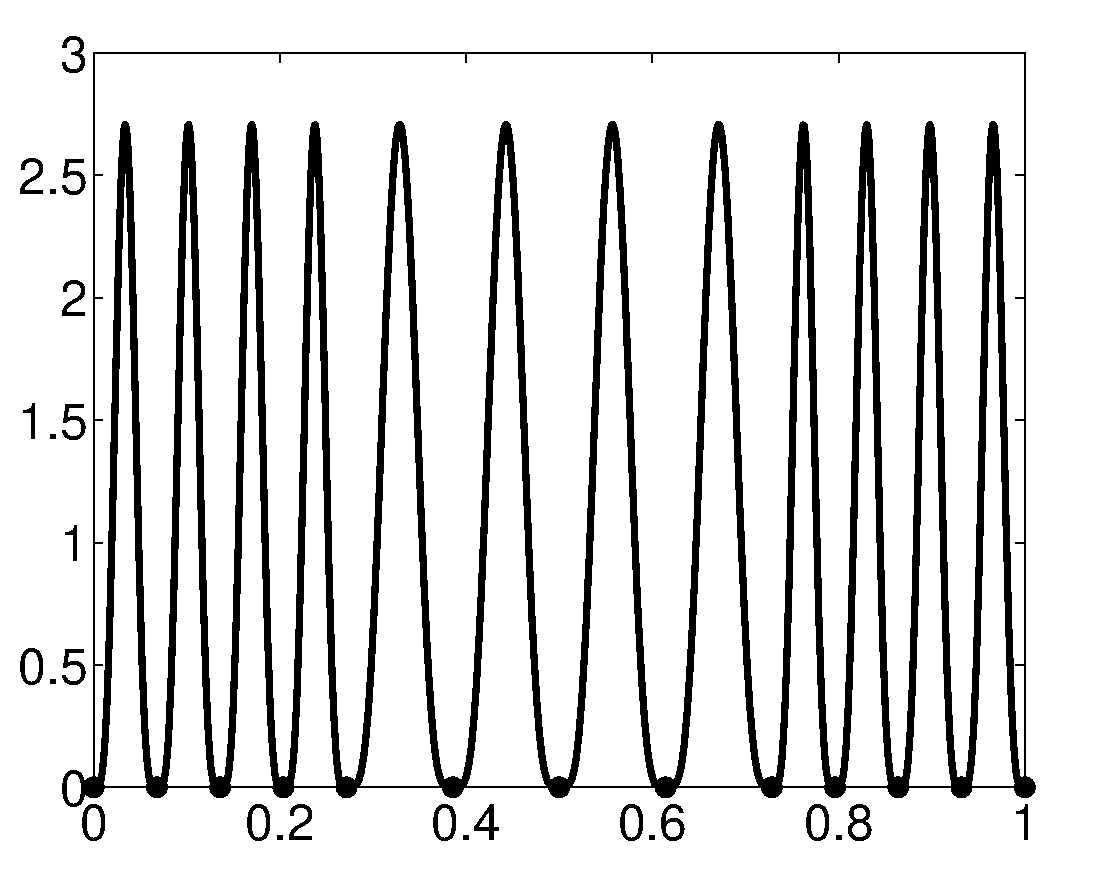
\includegraphics[width=3.7cm]{Foolquadbw.eps} \\ {\tt quad} \end{minipage}
\begin{minipage}{3.7cm} \centering 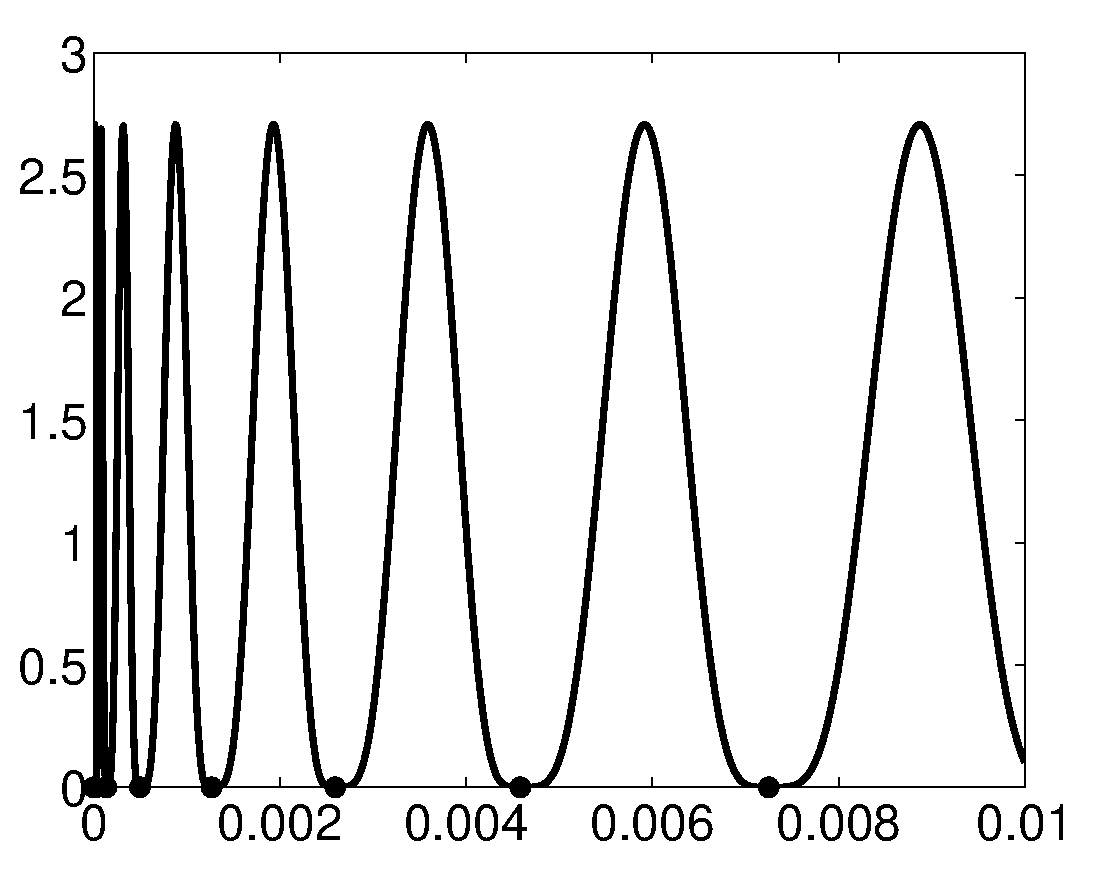
\includegraphics[width=3.7cm]{Foolquadgkbw.eps} \\ {\tt quadgk} \end{minipage}
\begin{minipage}{3.7cm} \centering 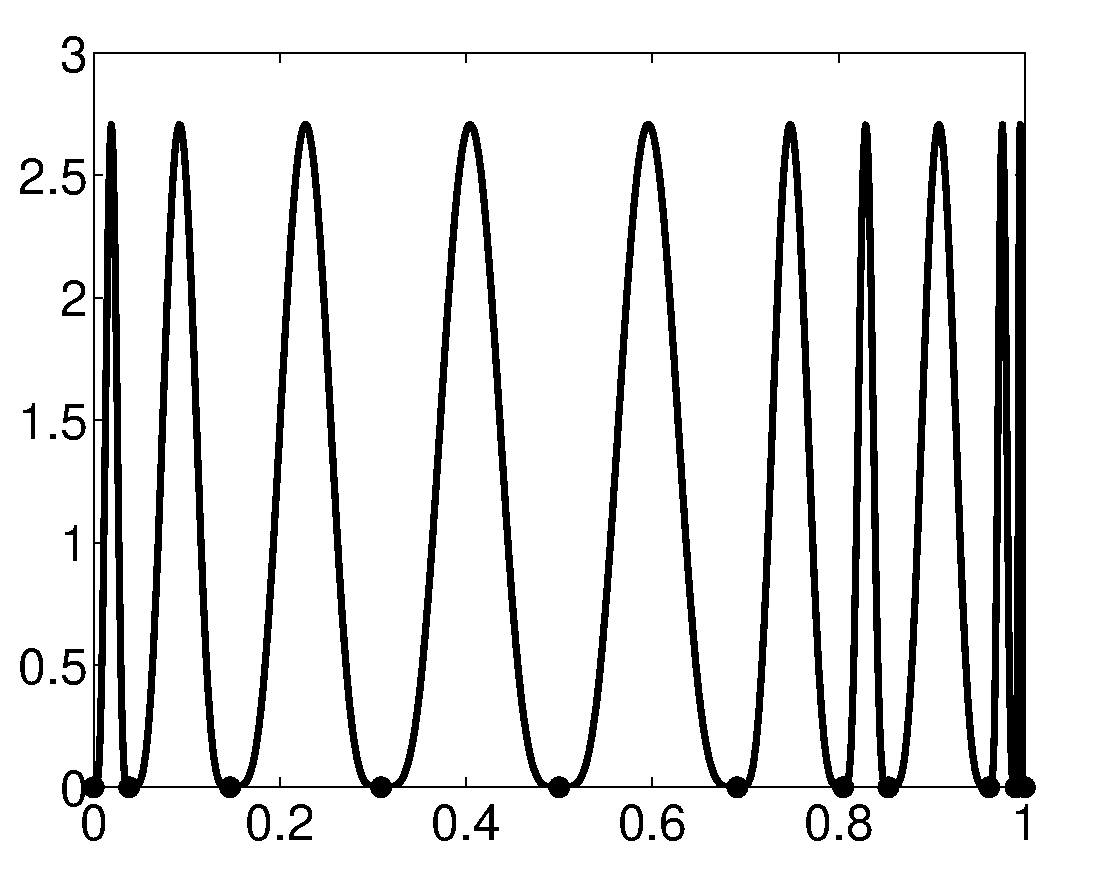
\includegraphics[width=3.7cm]{Foolchebintbw.eps} \\ {\tt chebfun} \end{minipage}
\caption{Plots of fooling functions, $f$, with $\mu=\int_0^1 f(x) \, \dif x=1$, but for which the corresponding algorithms return values of $\hmu=0$. \label{foolfunfig}}
\end{figure}

Another example is illustrated in Figure \ref{???} for the test function
\[
f(\vx) = b \exp\left(-\frac 12 [a_1^2(x_1-z_1)^2 + \cdots + a_1^2(x_1-z_1)^2]\right),
\]
and the integral $\mu=\int_{[0,1]^d} f(\vx) \, \dif \vx$.  The parameters are ....


\begin{figure}
\centering
\begin{minipage}{3.7cm} \centering 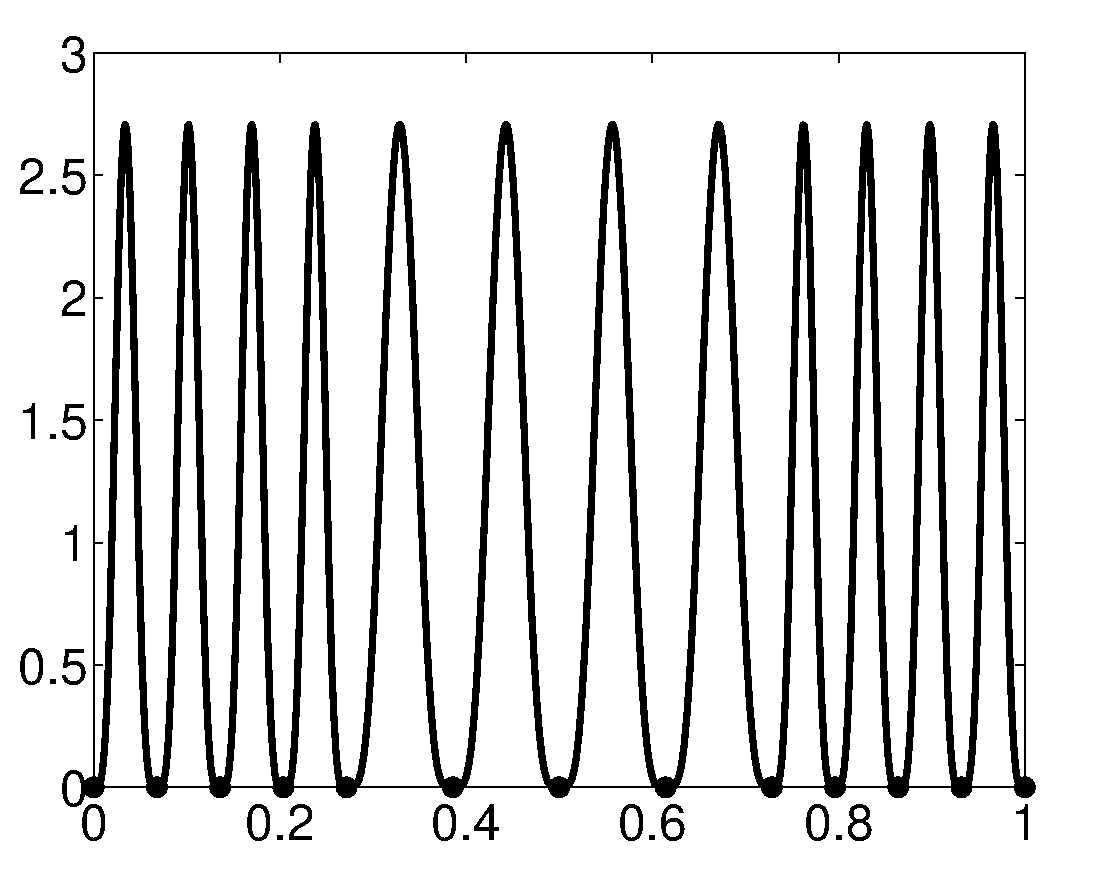
\includegraphics[width=3.7cm]{Foolquadbw.eps} \\ {\tt quad} \end{minipage}
\begin{minipage}{3.7cm} \centering 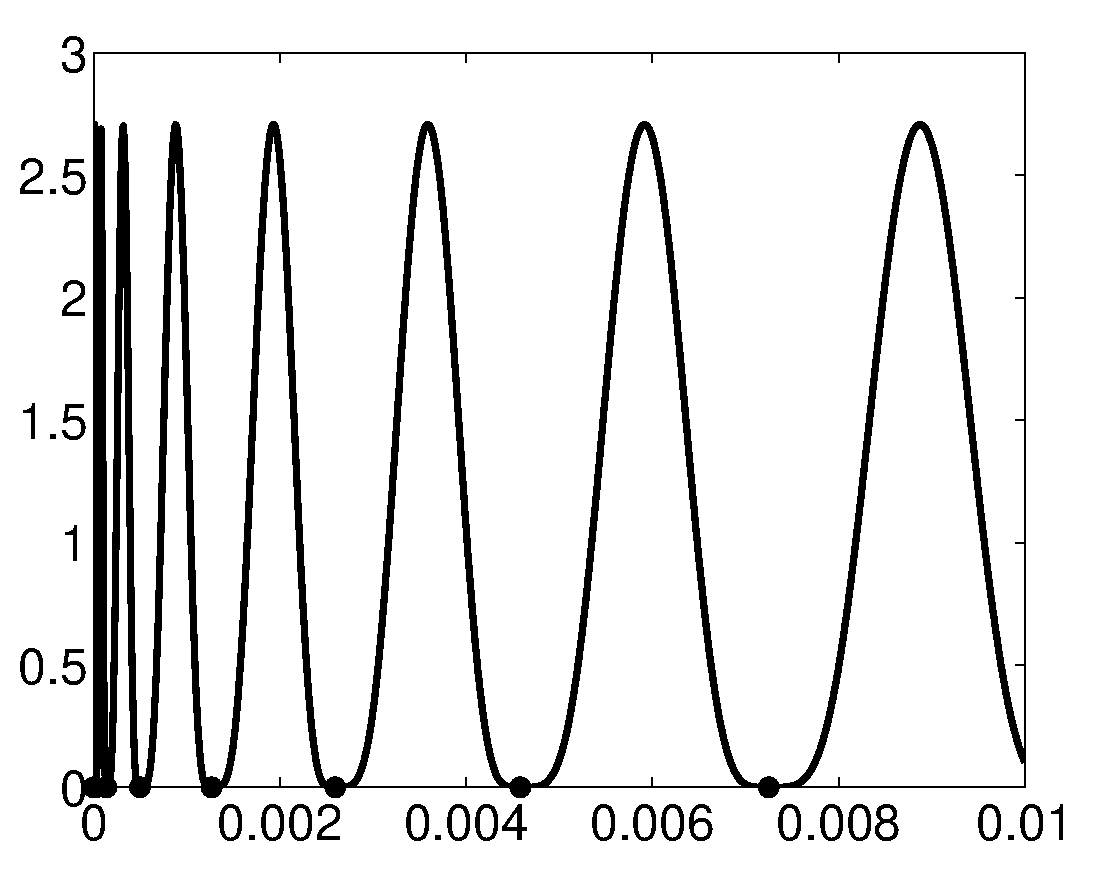
\includegraphics[width=3.7cm]{Foolquadgkbw.eps} \\ {\tt quadgk} \end{minipage}
\begin{minipage}{3.7cm} \centering 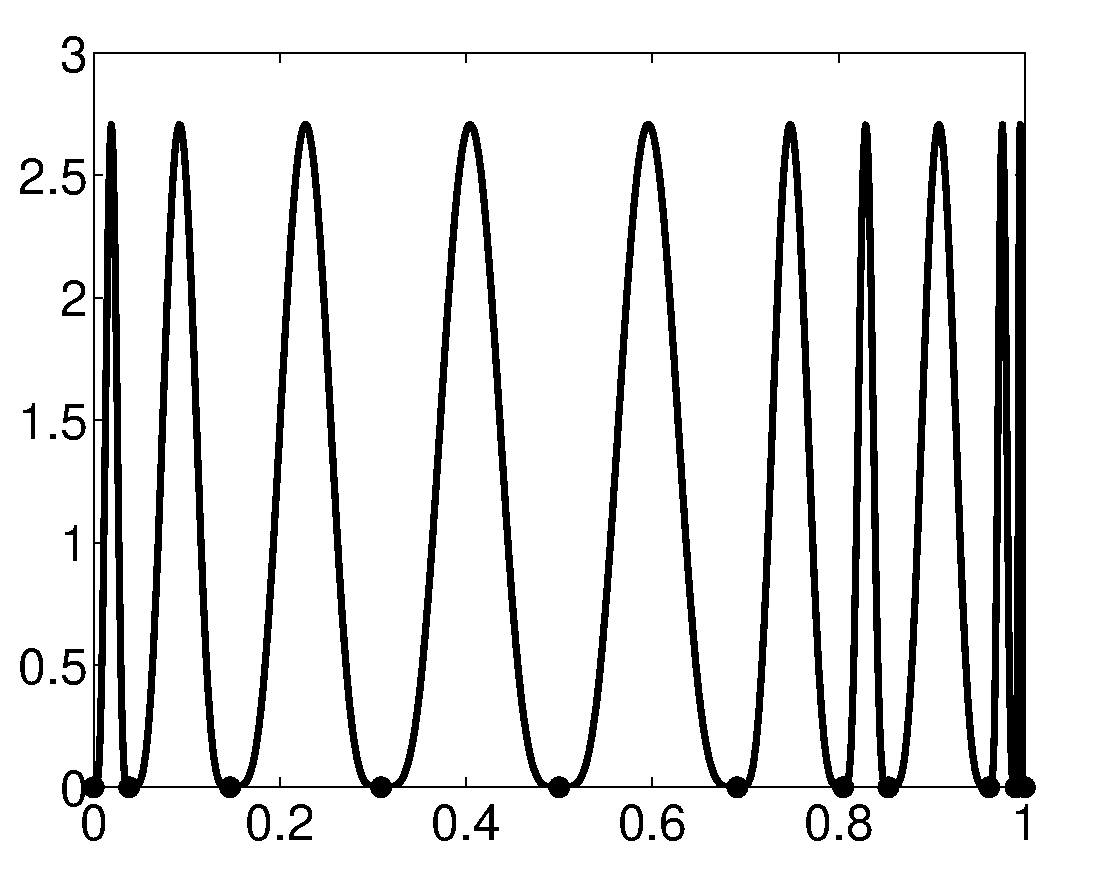
\includegraphics[width=3.7cm]{Foolchebintbw.eps} \\ {\tt chebfun} \end{minipage}
\caption{Execution times and errors for . \label{OneDGaussErrfig}}
\end{figure}



\section{Simple Monte Carlo with Guaranteed Error Estimation}

\subsection{Reliably Bounding the Variance} To estimate or bound the variance of $Y=f(\vX)$ one must have a finite fourth moment.  The definitions of the variance and kurtosis of $Y$ in Section \ref{statperspsec} may be extended naturally to $f \in \cl_4$ in terms of $\cl_p$ norms defined in \eqref{Lpnormdef} as follows:
\begin{equation*}
\sigma^2=\var(Y) = \var(f) = \norm[2]{f - \mu(f)}^2, \qquad \kappa=\kurt(Y) = \kurt(f) = \frac{\norm[4]{f - \mu(f)}^4}{\norm[2]{f - \mu(f)}^4}.
\end{equation*}
Thus, one may speak about $Y$ or $f$ interchangeably. If $1 \le q \le p$, then by H\"older's inequality,
\begin{align*}\label{LP}
\norm[q]{f} &=\left\{\int_{\reals^d} \abs{f(\vx)}^q \rho(\vx) \, \dif \vx\right\}^{1/q}\\
\nonumber & \le \left\{\int_{\reals^d} \abs{f(\vx)}^p \, \rho(\vx) \, \dif \vx \right\}^{1/p} \left\{\int_{\reals^d} 1^{p/(p-q)} \, \rho(\vx) \, \dif \vx\right\}^{(p-q)/(pq)} = \norm[p]{f}.
\end{align*}
Thus, $\kappa=\kurt(f) \ge 1$, provided $\sigma^2=\var(f)>0$.  For $\sigma^2=\var(f)=0$, one defines $\kappa=\kurt(f)=1$.

As mentioned in \eqref{samplevar}, a practical upper bound on $\sigma^2$ may be obtained in terms of the sample variance.  The justification for this statement is contained in the lemma below. Two well-known probability inequalities that are needed here and later are quoted in the following lemma.

\begin{lemma} \label{ChebCantlem}  Suppose that $Z$ is any random variable with finite second moment.  For any $a >0 $,
\begin{gather*}
\Prob\left[\abs{Z-E(Z)} \ge a \right] \le \frac{\var(Z)}{a^2} \qquad \text{Chebyshev's inequality \citep[6.1c]{LinBai10a}} , \\
\Prob[Z-E[Z] \geq a]\leq \frac{\var(Z)}{a^2+\var(Z)} \qquad
\text{Cantelli's Inequality \citep[6.1e]{LinBai10a}}.
\end{gather*}
\end{lemma}

\begin{lemma} \label{varbdlem}  Suppose that $Y$ is a random variable with finite fourth moment, and with mean $\mu$, variance $\sigma^2$, and kurtosis $\kappa$.  Let $\hv_{n}$ denote the unbiased sample variance based on $n$ i.i.d.\ samples, $Y_1, \ldots, Y_n$ as defined in \eqref{samplevar}.  Then for any $\alpha \in (0,1]$ it follows that
\begin{subequations} \label{sampvarbd}
\begin{gather} \label{sampvarup}
\Prob \left[\frac{\hv_{n}}{1 - \sqrt{\left ( \kappa  - \frac{n-3}{n-1}\right)\left(\frac{1-\alpha}{\alpha n}\right)}} > \sigma^2 \right] \ge 1 - \alpha, \\
\label{sampvarlo}
\Prob \left[\frac{\hv_{n}}{1 + \sqrt{\left ( \kappa  - \frac{n-3}{n-1}\right)\left(\frac{1-\alpha}{\alpha n}\right)}} < \sigma^2 \right] \ge 1 - \alpha.
\end{gather}
\end{subequations}
\end{lemma}

\begin{proof} It is known that the sample variance is an unbiased estimator of the variance, i.e., $E(\hv_n)=\sigma^2$.  It is also known from \cite{??} that the variance of the sample variance can be expressed in terms of $\sigma^2$ and $\kappa$ as
\[
\var(\hv_n) = \frac{\sigma^4}{n} \left ( \kappa  - \frac{n-3}{n-1} \right).
\]
Choosing
$$a=\sqrt{\var(\hv_n) \frac{1-\alpha}{\alpha} } = \sigma^2\sqrt{\left(\kappa-\frac{n-3}{n-1}\right)\left(\frac{1-\alpha}{\alpha n}\right)} >0,
$$
it follows from Cantelli's inequality (Lemma \ref{ChebCantlem})  that
\begin{multline*}
\Prob\left[\hv_n-\sigma^2 \geq
\sigma^2\sqrt{\left(\kappa-\frac{n-3}{n-1}\right)\left(\frac{1-\alpha}{\alpha n}\right)} \right]  = \Prob\left[\hv_n-\sigma^2 \geq
a \right]\\
 \leq \frac{\var(\hv_n)}{a^2+\var(\hv_n)} 
=\frac{\var(\hv_n)}{\var(\hv_n) \frac{1-\alpha}{\alpha}+\var(\hv_n)}  
=\frac{1}{\left(\frac{1-\alpha}{\alpha}\right)+1}=\alpha.
\end{multline*}
Then \eqref{sampvarup} follows directly.  By a similar argument, applying Cantelli's inequality to the expression $\Prob\left[-\hv_n+\sigma^2 \ge a \right]$ implies  \eqref{sampvarlo}. \qed
\end{proof}

Lemma \ref{varbdlem} provides probabilistic justification to use $\hsigma^2 = \fudge^2 \hv_{n_{\sigma}}$ as a reliable upper bound for $\sigma^2=\var(Y)=\var(f)$.  One can claim that $\Prob(\hsigma^2 \ge \sigma^2) \ge 1-\alpha$ assuming that
\begin{multline}
\frac{1}{1 - \sqrt{\left ( \kappa  - \frac{n_{\sigma}-3}{n_{\sigma}-1}\right)\left(\frac{1-\alpha}{\alpha n_{\sigma}}\right)}} \le \fudge^2
\\
\iff \kappa \le \frac{n_{\sigma}-3}{n_{\sigma}-1} + \left(\frac{ \alpha n_{\sigma}}{1-\alpha}\right) \left(1 - \frac{1}{\fudge^2}\right)^2 =: \kappa_{\max} (\alpha,n_{\sigma},\fudge). \label{kappamaxdef}
\end{multline}

Figure \ref{kurtmaxcompareNfig}a shows how large a kurtosis can be accommodated for a given $n_{\sigma}$, $\alpha$, and variance inflation factor $\fudge=1.5$.  Note that for $n=30$, a common rule of thumb for applying the central limit theorem, even $\alpha=0.1$ gives $\kappa_{\max}$ of only about $2$, which is rather restrictive.

\begin{figure}
\centering
\begin{minipage}{2.1in}
\centering 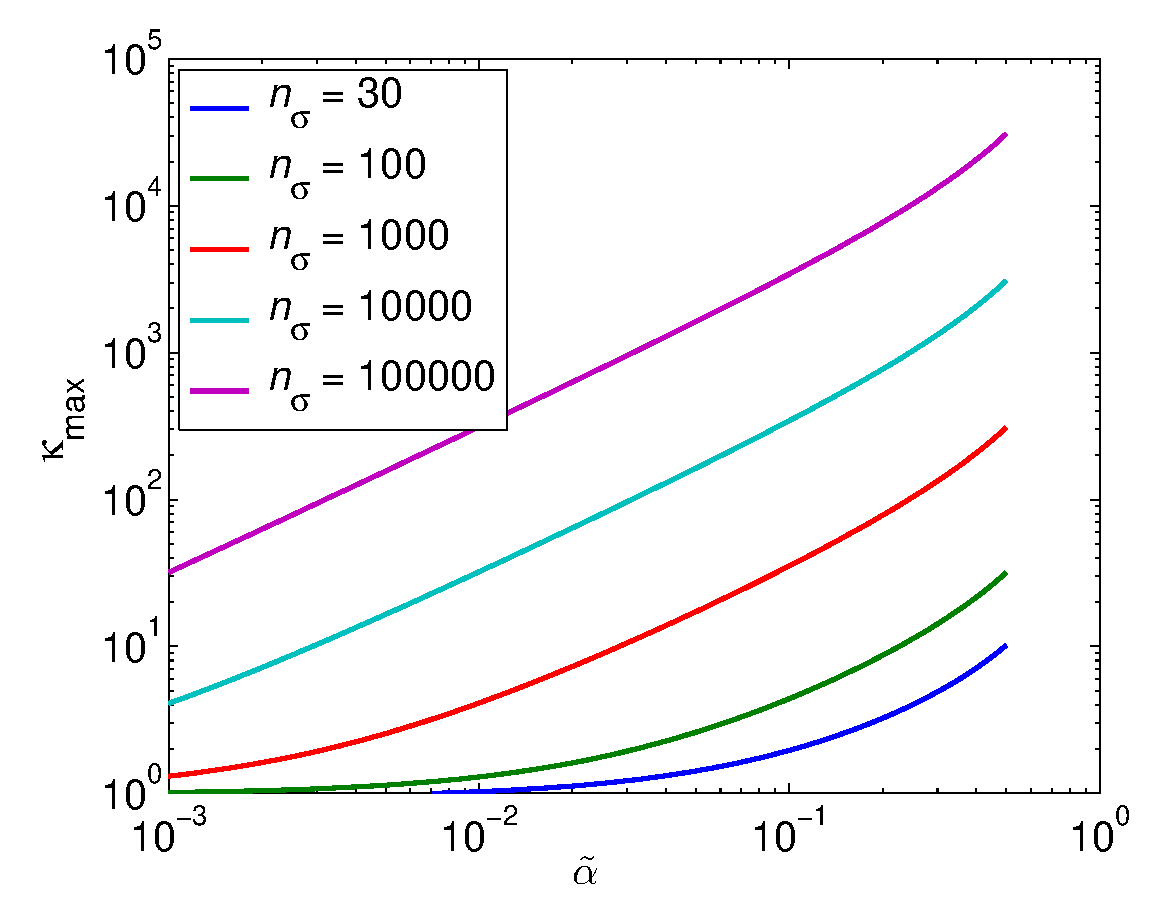
\includegraphics[width=2.1in]{kurtmaxfig.eps} \\
(a)
\end{minipage}
\quad 
\begin{minipage}{2.1in}\centering
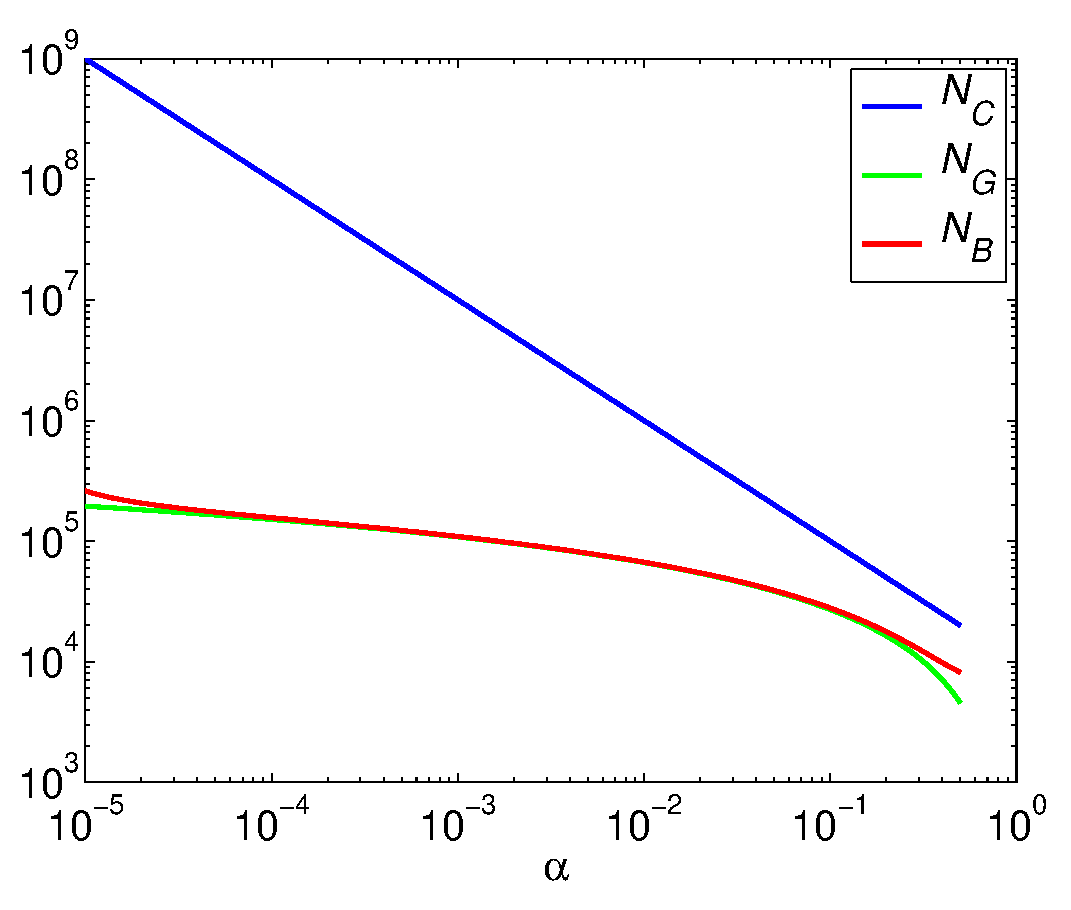
\includegraphics[width=2.1in]{alphacompare.eps}\\
(b)
\end{minipage}
\caption{(a) The maximum kurtosis, $\kappa_{\max}(\alpha,n_{\sigma},1.5)$, as defined in \eqref{kappamaxdef}; (b) comparison of sample sizes $ N_G(0.01,\alpha)$, $N_C(0.01,\alpha)$, and $N_B(0.01,\alpha,\kappa_{\max}^{3/4}(\alpha,1000,1.5))$.\label{kurtmaxcompareNfig}}
\end{figure}

\subsection{Determining the Sample Size} The other issue that needs to be addressed is a tight probabilistic error bound to replace the asymptotic or approximate error bound given by the Central Limit Theorem, \eqref{CLT}.   Chebyshev's inequality implies that the number of function evaluations needed to ensure that $\hmu_n$ satisfies the error tolerance with high probability is
\begin{subequations} \label{ChebErr}
\begin{gather} \label{ChebProbEst}
\Prob\left[\abs{\hmu_n-\mu} \le \varepsilon \right] \ge 1-\alpha \quad \text{for } n \ge N_{C}(\varepsilon/\sigma,\alpha),\ f \in \cl_2,
\intertext{where }
\label{NCdef}
N_{C}(\varepsilon,\alpha) :=\left \lceil \frac{1}{\alpha\varepsilon^2} \right \rceil.
\end{gather}
\end{subequations}
However, this sample size is much larger than that given by the Central Limit Theorem, as shown in Figure \ref{kurtmaxcompareNfig}b.

Since higher order moments of the integrand are required to guarantee an upper bound on the true variance in terms of the sample variance, it is sensible to use these higher order moments to obtain smaller sample sizes.  A smaller sample size than \eqref{NCdef} with a rigorous probabilistic bound can be found by invoking the following inequality. 
\begin{lemma}[Non-uniform Berry-Esseen Inequality] \cite[Theorem 5.16, p. 168]{Pet95a} \label{BE} Let $Y_1,\dots,Y_n$ be i.i.d.\ random variables.  Suppose that
$\mu=E(Y_i)$, $\var(Y_i)=\sigma^2>0$,  and $M=E\abs{Y_i - \mu}^3/\sigma^3 < \infty$.
Then
\[
\abs{\Prob\left[\frac{1}{\sigma\sqrt{n}}\sum_{i=1}^{n}(Y_i-\mu)<x
\right]-\Phi(x)}\leq \frac{A M}{\sqrt{n}(1+\abs{x})^{3}}.
\] for all x,
where $\Phi$ is the cumulative distribution function of a standard Gaussian (normal) random variable, and $A$ is some number satisfying $0.4097\leq A\leq 0.5600$.
\end{lemma}

The right hand side of this inequality bounds how far the probability distribution of sample mean deviates from the Central Limit Theorem approximation.  This right hand side vanishes as either the sample size or $\abs{x}$ tends to infinity. This inequality requires that $Y=f(\vX)$, have a finite third moment, i.e., $f \in \cl_3$, which is a weaker assumption than is needed to bound the variance in terms of the sample variance in Lemma \ref{varbdlem}. Recalling that $Y_i = f(\vX_i)$, $\mu=E(Y_i)$, and $\hmu_n =
(Y_1 + \cdots + Y_n)/n$, this
Berry-Esseen inequality then implies that for positive $x$,
\begin{align} 
\nonumber
\Prob\left[\abs{\hmu_n - \mu} <\frac{\sigma x}{\sqrt{n}}\right]&=\Prob\left[\hmu_n - \mu<\frac{\sigma x}{\sqrt{n}}\right]-\Prob\left[\hmu_n - \mu <-\frac{\sigma x}{\sqrt{n}}\right]\\
\nonumber
&\ge \left[\Phi(x)-\frac{0.56 M}{\sqrt{n}(1+\abs{x})^{3}}\right] -\left[\Phi(-x) + \frac{0.56 M}{\sqrt{n}(1+\abs{x})^{3}}\right]\\
&=1-2\left(\Phi(-x) - \frac{0.56 M}{\sqrt{n}(1+\abs{x})^{3}}\right). \label{BEresult}
\end{align}
Letting $x=\varepsilon\sqrt{n}/\sigma$, the probability of
making an error less than $\varepsilon$ is bounded below by $1-\alpha$, i.e., 
\begin{subequations} \label{proberrcritsampleBE}
\begin{equation}
\Prob[\abs{\hmu_n -\mu}<\varepsilon] \geq 1-\alpha,  \quad \text{provided } n \ge N_B(\varepsilon/\sigma,\alpha,M), \ f \in \cl_3,
\end{equation}
where 
\begin{equation}\label{NB}
N_B(b,\alpha,M) := \min \left \{ n \in \naturals : \Phi\left(-b \sqrt{n}  \right)+\frac{0.56M}{\sqrt{n}\left(1+ b\sqrt{n} \right)^{3}}
\le \frac{\alpha}{2} \right \}.
\end{equation}
\end{subequations}

As shown in Figure \ref{kurtmaxcompareNfig}b, for a range of $\alpha$, the sample size guaranteeing coverage of the confidence interval, $N_B$, is quite close to the sample size for the approximate Central Limit Theorem confidence interval, $N_G$, however, $N_B$ may be somewhat larger for very small or rather large $\alpha$.  In general $N_B$ is significantly smaller than $N_C$, but not always.  A disadvantage of \eqref{proberrcritsampleBE} is that class of integrands, $\cl_3$, is smaller than that in \eqref{ChebErr}, but this typically a small price to pay given the much smaller cost of computation.

The theorem below combines the results on estimating the variance with the sample sizes arising from Chebyshev's inequality and the Berry-Esseen inequality.  These lead to an adaptive Monte Carlo algorithm with a probabilistic error guarantee.

\begin{theorem} \label{mainadaptthm} Specify the following parameters defining the algorithm:
\begin{itemize}
\item sample size for variance estimation, $n_{\sigma} \in \naturals$,
\item inflation factor for variance estimation, $\fudge \in (1,\infty)$,
\item uncertainty tolerance, $\alpha\in (0,1)$, and $\talpha = 1 - \sqrt{1 - \alpha}$, and
\item absolute error tolerance, $\varepsilon \in (0,\infty)$. 
\end{itemize} 
For $\kappa_{\max}=\kappa_{\max}(n_{\sigma},\talpha,\fudge)$, as defined in \eqref{kappamaxdef}, define the cone of integrands functions with bounded kurtosis, $\cc_{\kappa_{\max}}$, according to \eqref{coneintegdef}.  For any $f \in \cc_{\kappa_{\max}}$, compute the sample variance, $\hv_{n_{\sigma}}$ using a simple random sample of size $n_{\sigma}$. Use this to approximate the variance of $f$ by $\hsigma^2 = \fudge^2 \hv_{n_{\sigma}}$ as in \eqref{samplevar}.  Next define a sample size $n = N_{CB}(\varepsilon/\hsigma,\talpha,\kappa_{\max}^{3/4})$, where
\begin{equation} \label{NCBdef}
N_{CB}(b,\alpha,M) := \min\left( N_C(b,\alpha), N_B(b,\alpha,M) \right),
\end{equation} 
$N_C$ is defined in \eqref{NCdef} and  $N_B$ is defined in \eqref{NB}.  Compute $\hmu_n$, the simple Monte Carlo estimator of $\mu$ based on $n$ samples, as in \eqref{simpleMCest}.  A probabilistic absolute error bound is given by
\[
\Prob\left[\abs{\hmu_n-\mu} \le \varepsilon \right] \geq 1-\alpha.
\]
\end{theorem}
\begin{proof} Note that \eqref{LP} implies that the third moment can be bounded in terms of the fourth moment, namely $M$ in Lemma \ref{BE} is no greater than $\kappa^{3/4}$. There are three primary random variables in this algorithm:  the estimated upper bound on the standard deviation, $\hsigma$, the sample size to estimate the mean, $n$, which is an explicit function of $\hsigma$, and the estimated mean, $\hmu_n$. By  \eqref{ChebErr} and \eqref{proberrcritsampleBE} it then follows that  $\Prob\left[\abs{\hmu_n-\mu} \le \varepsilon \right] \geq 1-\talpha$, provided that $\hsigma  \ge \sigma$. Thus, 
\begin{align*}
\Prob\left[\abs{\hmu_n-\mu} \le \varepsilon \right] &
= E_{\hsigma} \left\{\Prob\left[\abs{\hmu_n-\mu} \le \varepsilon \ | \ \hsigma \right] \right\} \\
& \ge E_{\hsigma} \left\{(1-\talpha) 1_{[\sigma,\infty)}(\hsigma) \right\}\\
& \ge (1-\talpha) (1-\talpha) = 1-\alpha,
\end{align*}
since $\hsigma \ge \sigma$ with probability $1-\talpha$ by \eqref{kappamaxdef}.  \qed
\end{proof}

\begin{rem} If one is willing to invest $n_\sigma$ samples to estimate $\sigma$, it makes practical sense to to choose the sample size for the sample mean at least that large, i.e, 
\[
n = \max(n_{\sigma},N_{CB}(\varepsilon/\hsigma,\talpha,\kappa_{\max}^{3/4})).
\]
By the error bound following from Chebyshev's inequality, \eqref{ChebErr}, this means that the probabilistic absolute error bound in Theorem \ref{mainadaptthm} also holds for integrands, $f$, lying in the ball $\cb_{\sigma_{\max}}$, defined in \eqref{ballintegdef}, where $\sigma_{\max} = \varepsilon \sqrt{\alpha n_{\sigma}}$ 
\end{rem}


\subsection{Cost of the Algorithm}  The sample size of the adaptive algorithm defined in Theorem \ref{mainadaptthm} is a random variable, and so the cost of this algorithm might best be defined defined probabilistically.  Moreover, the cost depends strongly on $\sigma$ as well as the $\varepsilon$, and its definition should reflect this dependence. 

Let $A$ be any random algorithm defined for a set of integrands $\cf$ that takes as its input an error tolerance, $\varepsilon$, an uncertainty level, $\alpha$, and a  procedure for computing values of $f \in \cf$.  The algorithm then computes an approximation to the integral, $A(f,\varepsilon,\alpha)$.  This approximation is based solely on  $f(\vx_1), \ldots, f(\vx_n)$, where the choice of each $\vx_i$ may depend iteratively on $(\vx_1,f(\vx_1)), \ldots, (\vx_{i-1},f(\vx_{i-1}))$, and the decision to stop with $n$ data depends on all function data collected, up to and including the $n^{\text{th}}$.  The cost of this algorithm for this set of inputs is denoted $\cost(A,\varepsilon,\alpha,f)$, is the number of function values, $n$, which as noted is a random variable.  The probabilistic cost of the algorithm, with uncertainty $\beta$, for integrands of variance no greater than $\sigma^2_{\max}$ is defined as 
\begin{equation}
\cost(A,\varepsilon,\alpha,\beta,\cf,\sigma_{\max}) := \sup_{\substack{f \in \cf\\ \var(f)\le \sigma^2} } \min\left\{N : \Prob[\cost(A,\varepsilon,\alpha,f) \le N] \ge 1-\beta  \right \}.
\end{equation}

The cost of the particular adaptive Monte Carlo algorithm defined in Theorem \ref{mainadaptthm}, denoted $\aMC$, for the cone of integrands $\cc_{\kappa_{\max}}$ is
\begin{equation}
\cost(\aMC,\varepsilon,\alpha, \beta, \cc_{\kappa_{\max}}, \sigma_{\max}) := \sup_{\substack{f \in \cc_{\kappa_{\max}}\\ \var(f)\le \sigma^2_{\max}} } \min\left\{N : \Prob(n_{\sigma} + n \le N) \ge 1-\beta  \right \}.
\end{equation}
Since $n_{\sigma}$ is fixed, bounding this cost depends on bounding $n$, which depends on $\hsigma$ as given by Theorem \ref{mainadaptthm}.  Moreover, $\hsigma$ can be bounded above using \eqref{sampvarlo} in Lemma \ref{varbdlem}.  For $f \in \cc_{\kappa_{\max}}$, 
\begin{align*}
1-\beta & \le \Prob\left[\hv_{n_{\sigma}} < \sigma^2 \left\{1 + \sqrt{\left ( \kappa  - \frac{n_{\sigma}-3}{n_{\sigma}-1}\right)\left(\frac{1-\beta}{\beta n_{\sigma}}\right)}\right\} \right] \\
& \le \Prob\left[\hsigma^2 = \fudge^2 \hv_{n_{\sigma}} < \fudge^2\sigma^2 \left\{1 + \sqrt{\left ( \kappa_{\max}(n_{\sigma},\talpha,\fudge)  - \frac{n_{\sigma}-3}{n_{\sigma}-1}\right)\left(\frac{1-\beta}{\beta n_{\sigma}}\right)}\right\} \right] \\
%& = \Prob\left[\hsigma^2 < \fudge^2\sigma^2 \left\{1 + \sqrt{\left(\frac{ \talpha }{1-\talpha}\right) \left(\frac{1-\beta}{\beta}\right) \left(1 - \frac{1}{\fudge^2}\right)^2}\right\} \right] \\
& = \Prob\left[\hsigma^2 < \sigma^2 \gamma^2(\talpha,\beta,\fudge) \right],
\end{align*}
where
\[
\gamma^2(\talpha,\beta,\fudge) := \fudge^2 \left\{1 + \sqrt{\left(\frac{ \talpha }{1-\talpha}\right) \left(\frac{1-\beta}{\beta}\right) \left(1 - \frac{1}{\fudge^2}\right)^2}\right\} > 1.
\]
Noting that $N_{CB}(\cdot,\alpha,M)$ is a non-increasing function allows one to derive the following upper bound on the cost of the adaptive Monte Carlo algorithm.

\begin{theorem} \label{costtheorem} The adaptive Monte Carlo algorithm described in Theorem \ref{mainadaptthm}, denoted $\aMC$, has a probabilistic cost bounded above by 
\begin{equation*}
\cost(\aMC,\varepsilon,\alpha, \beta, \cc_{\kappa_{\max}}, \sigma_{\max})
\le n_{\sigma} + N_{CB}(\varepsilon/(\sigma_{\max}\gamma(\talpha,\beta,\fudge)),\talpha,\kappa_{\max}^{3/4}).
\end{equation*} 
\end{theorem}

The cost of the adaptive Monte Carlo algorithm $\aMC$ is roughly proportional to $\sigma^2_{\max}\varepsilon^{-2}$.  The set $\cc_{\kappa_{\max}}$ contains integrands with arbitrarily large variance, $\sigma^2=\var(f)$, and thus with potentially arbitrarily large algorithmic cost.  On the other hand, since the algorithm is adaptive, the cost may be small if $\sigma^2$ is small.  The upper bound in Theorem \ref{costtheorem} certainly scales with the $\sigma^2_{\max}$ as one might hope if $\sigma^2_{\max}$ were known.  The variable cost of the algorithm for integrands in $\cc_{\kappa_{\max}}$ is actually an advantage, rather than a drawback, of this analysis.  One need not make any a priori assumptions about the size of the integrand, $\sigma$, only about its kurtosis, $\kappa$, which is unchanged when the integrand is multiplied by an arbitrary nonzero constant.

\section{Simple Monte Carlo Satisfying a Relative Error Criterion} \label{relerrsec}

In many practical situations, one needs to approximate the integral with a certain relative accuracy.  For example, one wants an answer that is correct to three significant digits.  In this case, given a tolerance, $\varepsilon$, and a significance level $\alpha$, with $\varepsilon, \alpha \in (0, 1)$, one seeks a random $\tmu$ such that 
\begin{equation} \label{relerrcrit}
\Prob\left[\abs{\frac{\tmu-\mu}{\mu}} \le \varepsilon \right] \geq 1-\alpha.
\end{equation}
A more general form of this criterion would be
\begin{equation} \label{genrelerrcrit}
\Prob\left[\frac{\abs{\tmu-\mu}} {1-\theta + \theta\abs{\mu}} \le \varepsilon \right] \geq 1-\alpha.
\end{equation}
for some fixed $\theta \in [0,1]$, where $\theta=0$ corresponds to absolute error, and $\theta = 1$ corresponds to relative error.
Clearly, one must have $(1-\theta) + \abs{\mu}\ne0$ for such a statement to be possible.  


The above form is not a traditional confidence interval, however, suppose that one has the following confidence interval for $\mu$ in terms of $\hmu$ and $\hvareps$: 
\begin{equation} \label{relerrcritc}
1-\alpha \le \Prob\left[\abs{\hmu-\mu} \le \hvareps \right] = \Prob[\hmu-\hvareps \le \mu \le \hmu+\hvareps].
\end{equation}
Define $\tmu$ and $\tvareps>0$ to satisfy
\begin{gather}
\label{tmudef}
\frac{\tmu \pm (1-\theta) \tvareps}{1 \mp \theta \tvareps \sign(\hmu \mp \hvareps)} = \hmu \pm \hvareps \\
\nonumber
\iff \tmu \pm (1-\theta) \tvareps = (\hmu \pm \hvareps)[1 \mp \theta \tvareps \sign(\hmu \mp \hvareps)] \\
\nonumber
\iff \tmu \pm [(1-\theta) + \theta\sign(\hmu \mp \hvareps)(\hmu \pm \hvareps)]\tvareps = (\hmu \pm \hvareps) \\
\nonumber
\iff \begin{cases}
\displaystyle \tvareps= \frac{\hvareps}{1 -\theta +\frac{\theta}{2}[\sign(\hmu-\hvareps)(\hmu+\hvareps) + \sign(\hmu+\hvareps)(\hmu-\hvareps)]}\\[3ex]
\displaystyle \tmu= \hmu - \frac{\theta\tvareps}{2}[\sign(\hmu-\hvareps)(\hmu+\hvareps) - \sign(\hmu+\hvareps)(\hmu-\hvareps)] 
\end{cases}\\
\label{tepsdefb}
\iff 
\left\{
\begin{array}{lll}
\displaystyle \tvareps= \frac{\hvareps}{1 -\theta - \theta\hvareps}, & 
\displaystyle \tmu
%= \hmu + \theta\tvareps\hmu 
= \frac{\hmu(1-\theta)}{1 -\theta - \theta\hvareps}, &
\abs{\hmu} < \hvareps, \\[2ex]
\displaystyle \tvareps= \frac{\hvareps}{1 -\theta}, & 
\tmu= \hmu, & 
\abs{\hmu} = \hvareps,\\[2ex]
\displaystyle \tvareps= \frac{\hvareps}{1 -\theta + \theta\abs{\hmu}}, & 
\displaystyle \tmu
%= \hmu - \theta\tvareps\sign(\hmu)\hvareps 
= \frac{\hmu(1 -\theta) + \theta(\hmu^2-\hvareps^2)\sign(\hmu)}{1 -\theta + \theta\abs{\hmu}}, & 
\abs{\hmu} > \hvareps.
\end{array}
\right.
\end{gather}
Here, one must have $\hvareps<\min(\abs{\hmu},(1-\theta)/\theta)$ to ensure that $\tvareps$ is positive. 

Based on these definitions of $\tmu$ and $\tvareps>0$, it then follows from the confidence interval \eqref{relerrcritc} that 
\begin{align}
\nonumber
1- \alpha & 
\le \Prob[\hmu-\hvareps \le \mu \le \hmu+\hvareps]\\
\nonumber
& = \Prob\left[ \frac{\tmu-(1-\theta)\tvareps}{1+\theta\tvareps\sign(\hmu+\hvareps)} \le \mu \le \frac{\tmu + (1-\theta) \tvareps}{1-\theta\tvareps\sign(\hmu-\hvareps)} \right] 
\qquad \text{by \eqref{tmudef}} \\
\nonumber
& = \Prob\left[ \tmu-(1-\theta)\tvareps \le \mu[1+\theta\tvareps\sign(\hmu+\hvareps)] \  \& \right. \\
\nonumber
& \qquad \qquad \left .  \mu[1-\theta\tvareps\sign(\hmu-\hvareps)] \le \tmu + (1-\theta) \tvareps \right] \qquad \text{since $\tvareps<1/\theta$ for $\abs{\hmu} > \hvareps$}\\
\nonumber
& = \Prob\left[ -\{1-\theta + \theta\mu\sign(\hmu+\hvareps)\} \tvareps \le \mu - \tmu \le  \{1-\theta + \theta\mu\sign(\hmu+\hvareps)\}\tvareps \right] \\
\nonumber
& \le \Prob\left[ -(1-\theta + \theta\abs{\mu}) \tvareps \le \mu - \tmu \le  (1-\theta + \theta\abs{\mu})\tvareps \right] \qquad \text{by \eqref{relerrcritc}},
\end{align}
which implies the generalized confidence interval, \eqref{genrelerrcrit}, provided that $\tvareps \le \varepsilon$.  The previous section shows how to find absolute error criteria of the form \eqref{relerrcritc}, but the challenge is to ensure that $\tvareps$, as defined in \eqref{tepsdefb} in terms of $\hmu$ and $\hvareps$, is no greater than the specified $\varepsilon$. This is done iteratively as described in Theorem \ref{relerradaptthm} below.

Some notation is needed for this theorem.  For any fixed $\alpha \in (0,1)$, and $M>0$, define the inverse of the functions $N_C(\cdot,\alpha)$, $N_B(\cdot,\alpha,M)$, and $N_{CB}(\cdot,\alpha,M)$,
\begin{subequations} \label{probadapterrcritBE}
\begin{gather}\label{NCinv}
N_C^{-1}(n,\alpha) := \frac{1}{\sqrt{n \alpha}}, \\
\label{NBinv}
N_B^{-1}(n,\alpha,M) := \min \left \{ b>0 : \Phi\left(-b \sqrt{n}  \right)+\frac{0.56M}{\sqrt{n}\left(1+ b\sqrt{n} \right)^{3}}
\le \frac{\alpha}{2} \right \}, \\
\label{NCBinv}
N_{CB}^{-1}(n,\alpha,M) := \min(N_C^{-1}(n,\alpha),N_B^{-1}(n,\alpha,M)).
\end{gather}
It then follows then by Chebyshev's inequality and the Berry-Esseen Inequality (see \eqref{BEresult}) that 
\begin{equation}
\Prob[\abs{\hmu_n -\mu}<\hvareps] \geq 1-\alpha, \quad \text{provided } \ f \in \cc_{\kappa_{\max}}, \text{ where }\hvareps=\sigma(f) N_{CB}^{-1}(n,\alpha,\kappa_{\max}^{3/4}), 
\end{equation} 
\end{subequations}
and $\sigma(f)=\sqrt{\var(f)}$ is the standard deviation of the integrand.  Given a significance level, $\alpha \in (0,1)$, let $\alpha_{\sigma}, \alpha_1,  \alpha_2, \ldots$ be an infinite sequence of positive numbers all less than one, such that 
\begin{equation} \label{alphaseq}
(1-\alpha_{\sigma})(1-\alpha_1)(1-\alpha_2) \cdots = 1-\alpha.
\end{equation}
For example, one might choose
\begin{equation} \label{alphaseqex}
\alpha_{\sigma} = 1-\me^{-a_2}, \ \ \alpha_{i} = 1-\me^{-a_2a_1^{-i}}, \ i\in \naturals, \quad \text{where} \  a_1 \in (1,\infty), \  b_2=\frac{1-a}{a} \log(1-\alpha).
\end{equation}

\begin{theorem} \label{relerradaptthm} Specify the following parameters defining the algorithm:
\begin{itemize}
\item sample size for variance estimation, $n_{\sigma} \in \naturals$,
\item initial sample size for mean estimation, $n_1 \in \naturals$,
\item variance inflation factor for variance estimation, $\fudge \in (1,\infty)$, 
\item factor for confidence interval width reduction, $\delta \in (0,1)$,
\item uncertainty tolerance, $\alpha\in (0,1)$, and a sequence $\alpha_{\sigma}, \alpha_1,  \alpha_2, \ldots$ satisfying \eqref{alphaseq}, and
\item relative error tolerance, $\varepsilon \in (0,1)$. 
\end{itemize} 
Define the set of functions with bounded kurtosis and nonzero mean:
\[
\cc_{\kappa_{\max},0}= \{f \in \cl_{4} : \kurt(f)= \kappa \le \kappa_{\max}(n_{\sigma},\alpha_{\sigma},\fudge), \mu(f) \ne 0\},
\]
where $\kappa_{\max}$ is defined in \eqref{kappamaxdef}.  For any $f \in \cc_{\kappa_{\max},0}$, compute the sample variance, $\hv_{n_{\sigma}}$ using a simple random sample of size $n_{\sigma}$. Use this to approximate the variance of $f$ by $\hsigma^2 = \fudge^2 \hv_{n_{\sigma}}$, as in \eqref{sigmadef}, and to compute the width of initial the confidence interval for the mean, $\tvareps_1=\hsigma N_{CB}^{-1}(n_1,\alpha_1,\kappa_{\max}^{3/4})$.  For $i=1, 2, \ldots$, do the following:
\begin{enumerate}
\renewcommand{\labelenumi}{\alph{enumi})}
\item Compute the sample average $\hmu_{n_i}$ using a simple random sample that is independent of those used to compute $\hv_{n_{\sigma}}$ and $\hmu_{n_1}, \ldots, \hmu_{n_{i-1}}$.

\item If $\tvareps_i > \varepsilon \abs{\hmu_{n_i}}$, then reduce the width of the next confidence interval for the mean, 
\[
\tvareps_{i+1} = \min(\delta\tvareps_i, \varepsilon \max(\tvareps_i,\abs{\hmu_{n_i}}-\tvareps_i)).
\]
Define the next sample size, $n_{i+1} = N_{CB}(\tvareps_{i+1}/\hsigma,\alpha_{i+1},\kappa_{\max}^{3/4})$,
increase $i$ by one, and go to step a). 

\item Else, let $\tmu = \hmu_{n_i}(1 - \tvareps_i^2/\hmu_{n_i}^2)$, and terminate the algorithm because the relative error criterion, \eqref{relerrcrit}, is satisfied.

\end{enumerate}
\end{theorem}

\begin{proof} In this algorithm there are a number of important random variables:  the estimated upper bound on the standard deviation, $\hsigma$, the sample sizes $n_1, \ldots, n_\tau$, the number of confidence intervals computed, $\tau$, and the estimates of the mean, $\hmu_{n_1}, \ldots, \hmu_{n_{\tau}}$. These sample means are conditionally independent given the sequence of sample sizes.  The probability that the final confidence interval is correct, is then no less than the probability that all of the confidence intervals are correct, conditioned on the sample sizes.  Specifically,
\begin{align*}
\Prob\left[\abs{\frac{\tmu-\mu}{\mu}} \le \varepsilon \right] & 
\ge \Prob\left[\abs{\hmu_{n_{\tau}}-\mu} \le \tvareps_{n_{\tau}} \ \& \ \varepsilon \hmu_{n_{\tau}} \le \tvareps_{n_{\tau}} \right] \\
& = E \left\{\Prob\left[\abs{\hmu_{n_{\tau}}-\mu} \le \tvareps_{n_{\tau}} \ \& \ \varepsilon \hmu_{n_{\tau}} \le \tvareps_{n_{\tau}} \ | \ \hsigma, \tau, n_1, \ldots, n_{\tau} \right] \right\} \\
& \ge E \left\{\Prob\left[\abs{\hmu_{n_{i}}-\mu} \le \tvareps_{n_{i}}] \forall i \ \& \ \varepsilon \hmu_{n_{\tau}} \le \tvareps_{n_{\tau}} \ | \ \hsigma, \tau, n_1, \ldots, n_{\tau} \right] \right\} \\
& \ge E_{\hsigma} \left\{[(1-\alpha_1)(1-\alpha_2) \cdots] 1_{[\sigma,\infty)}(\hsigma) \right\}\\
& \ge (1-\alpha_{\sigma}) (1-\alpha_1)(1-\alpha_2) \cdots = 1-\alpha. \qquad \qed
\end{align*}
\end{proof}


\section{Numerical Examples}

\section*{Acknowledgements} The authors gratefully acknowledge discussions with Erich Novak and Henryk Wo\'zniakowski.

\bibliographystyle{spbasic}
\bibliography{FJH22,FJHown22}
\end{document}

\begin{prop}\label{latnetprop} For the situation described in Section \ref{qmcsec} with the operations $\oplus$, $\ominus$, and $\otimes$, the basis functions $\phi_{\vk}$, and any $\oplus$-closed set, $P$, with cardinality $\abs{P}$ and associated dual lattice $P^{\perp}$, it follows that 
\begin{gather}
\label{basisorth}
\mu(\phi_{\vk})= \int_{\cube} \phi_{\vk}(\vx) \, \dif \vx = \int_{\cube} e^{2 \pi \sqrt{-1} \vk \otimes \vx} \, \dif \vx = \delta_{\vk, \vzero}, \\
\label{duallatorth}
Q(\phi_{\vk},P,\vDelta)= \frac{1}{\abs{P}}\sum_{\vx \in P} \phi_{\vk}(\vx \oplus \vDelta) = \begin{cases} \phi_{\vk}(\vDelta), & \vk \in P^{\perp} \\ 0, & \vk \notin P^{\perp}
\end{cases}
\end{gather}
\end{prop}
\begin{proof}
The properties assumed for the binary operations imply that for all $\vt \in \cube$,
\begin{align*}
\int_{\cube} \phi_{\vk}(\vx) \, \dif \vx &= \int_{\cube} \phi_{\vk}(\vx \oplus \vt) \, \dif \vx = \phi_{\vk}(\vt) \int_{\cube} \phi_{\vk}(\vx) \, \dif \vx\\
0 & = \left [\phi_{\vk}(\vt) -1 \right] \int_{\cube} \phi_{\vk}(\vx) \, \dif \vx
\end{align*}
This inequality is satisfied iff $\vk=\vzero$ or $\int_{\cube} \phi_{\vk}(\vx) \, \dif \vx =0$.  This establishes \eqref{basisorth}. 

A similar argument establishes \eqref{duallatorth}.  Note first that the sum can be simplified to a multiple of $\phi_{\vk}(\vDelta)$:
\begin{equation*}
\frac{1}{\abs{P}}\sum_{\vx \in P} \phi_{\vk}(\vx \oplus \vDelta) 
= \frac{1}{\abs{P}}\sum_{\vx \in P} [\phi_{\vk}(\vx) \phi_{\vk}(\vDelta)] = \phi_{\vk}(\vDelta) \frac{1}{\abs{P}}\sum_{\vx \in P} \phi_{\vk}(\vx).
\end{equation*}
Next, note that for all $\vt \in P$ the remaining sum above is unchanged when the argument of $\phi_{\vk}$ is shifted by $\vt$:
\begin{align*}
\frac{1}{\abs{P}}\sum_{\vx \in P} \phi_{\vk}(\vx) 
& = \frac{1}{\abs{P}}\sum_{\vx \in P} \phi_{\vk}(\vx+\vt) 
= \frac{1}{\abs{P}}\sum_{\vx \in P} [\phi_{\vk}(\vx) \phi_{\vk}(\vt)] 
= \phi_{\vk}(\vt) \frac{1}{\abs{P}}\sum_{\vx \in P} \phi_{\vk}(\vx),\\
0 & = \left (\phi_{\vk}(\vt) -1 \right) \frac{1}{\abs{P}}\sum_{\vx \in P} \phi_{\vk}(\vx).
\end{align*}
This inequality is satisfied iff $\phi_{\vk}(\vt)=0$ for all $\vt \in P$, i.e., $\vk \in P^{\perp}$, or $\sum_{\vx \in P} \phi_{\vk}(\vx) =0$.  This implies \eqref{duallatorth}. \qed
\end{proof}


\section{Quasi-Standard Error Estimation for Quasi-Monte Carlo Methods} \label{qmcrepsec}

Quasi-Monte Carlo methods utilize low discrepancy node sets, in particular integration lattices and digital nets, to expedite the convergence of the sample mean to the true mean the sample size increases.  Like the case of i.i.d.\ sampling discussed in the previous section, one is faced with the question of how to choose the sample size in a data-driven way.

One way used in practice is to compute independent randomizations of the low discrepancy sequence.  This means replacing $Y_i=f(\vX_i)$ in the equation for the sample mean, \eqref{simpleMCest}, and the equation for the variance estimate, \eqref{samplevar}, which are used to define the adaptive algorithm of Theorem \ref{mainadaptthm}, by
\[
Y_i = \frac{1}{n_1} \sum_{j=1}^{n_1} f(\vZ_{ij}).
\]
Here the set $\{\vZ_{i1},\ldots, \vZ_{in_1}\}$ is the $i^{\text{th}}$ independent randomization (replication) of an integration lattice or net with $n_1$ points.  

If $n_1$ is fixed, then Theorems \ref{mainadaptthm} and \ref{costtheorem} may be extended in a natural way.  Now the number of integrand values required is $n_1$ times what the formulas in those theorems state, however, the total cost in practice may well be less than simple Monte Carlo because the sample variance using $n_{\sigma}$ replications of a low discrepancy node set with $n_1$ points may be much smaller than the corresponding sample variance using i.i.d.\ sampling with $n_{\sigma}n_1$ integrand values.  However, for this approach of fixed $n_1$, the sample variance only tells you how to choose \emph{more replications}.  It cannot tell you how to increase the size of the low discrepancy set while keeping the number of replications fixed.  Thus, the benefits of quasi-Monte Carlo methods are not fully realized.  

If the size of the low discrepancy set is increased until the error tolerance is met, then the algorithm becomes somewhat more complex.  Let, $n_1, n_2, \dots$ be a sequence of sample sizes for which one may obtain low discrepancy node sets.  Moreover, let $\alpha_{11}, \ $

Here there is an additional challenge.  

\section{Quasi-Standard Error Estimation for Quasi-Monte Carlo Methods} \label{qmcqsesec}

An alternative is to use the \emph{quasi-standard error}, also called \emph{internal replications} to estimate the error and then determine a reasonable sample size.  The quasi-standard error has been proposed by \cite{Hal05a}, but its implementation and justification have been criticized by \cite{Owe06a}.  A closer look at the quasi-standard error specifically applied to lattices and nets is provided here. 

Integration lattices {\bf references} A general framework that encompasses both kinds of designs is employed so that the analysis of both can be combined.  Table \ref{discdestab} provides the definitions for the general notation introduced below.  For integration lattices the operations are done with modulo arithmetic, and for digital nets they are done with $b$-ary digit-wise arithmetic.

\begin{table}
\caption{Definitions for low discrepancy designs for $x,t \in [0,1)$, $\vx,\vt \in \cube$, $k, l \in \Omega^d$ and $\vk, \vl \in \Omega^d$ \label{discdestab}}
\renewcommand{\arraystretch}{1.5}
\[
\begin{array}{c@{\qquad}c}
\text{Integration Lattices} & \text{Digital Nets in Base } b\\
\toprule
x \oplus t := x + t \bmod 1  & \displaystyle x \oplus t =\sum_{\ell=1}^\infty x_{\ell}b^{-\ell} \oplus \sum_{\ell=1}^\infty t_{\ell}b^{-\ell} := \sum_{\ell=1}^\infty (x_{\ell} + t_{\ell} \bmod b) b^{-\ell} \pmod 1\\
\ominus x := 1-x \bmod 1  & \displaystyle \ominus \sum_{\ell=1}^\infty x_{\ell}b^{-\ell}  := \sum_{\ell=1}^\infty (b - x_{\ell} \bmod b) b^{-\ell} \pmod 1\\
\multicolumn{2}{c}{\vx \oplus \vt= (x_1, \ldots, x_d) \oplus (t_1, \ldots, t_d) = (x_1 \oplus t_1, \ldots, x_d \oplus t_d)} \\
\multicolumn{2}{c}{\ominus\vx = \ominus (x_1, \ldots, x_d) = (\ominus x_1, \ldots, \ominus x_d)} \\
\midrule
\Omega:=\integers  & \Omega := \naturals_0 \\
k \oplus l := k + l &  
\displaystyle k \oplus l =\sum_{\ell=0}^\infty k_{\ell}b^{\ell} \oplus \sum_{\ell=0}^\infty l_{\ell}b^{\ell} := \sum_{\ell=0}^\infty (k_{\ell} + l_{\ell} \bmod b) b^{\ell}\\
\ominus k := -k & 
\displaystyle \ominus k = \ominus \sum_{\ell=0}^\infty k_{\ell}b^{\ell} := \sum_{\ell=0}^\infty (b - k_{\ell} \bmod b) b^{\ell}\\
\multicolumn{2}{c}{\vk \oplus \vl= (k_1, \ldots, k_d) \oplus (l_1, \ldots, l_d) = (k_1 \oplus l_1, \ldots, k_d \oplus l_d)} \\
\multicolumn{2}{c}{\ominus\vk = \ominus (k_1, \ldots, k_d) = (\ominus k_1, \ldots, \ominus k_d)} \\
\midrule
k \otimes x = kx \bmod 1 & \displaystyle k \otimes x =\sum_{\ell=0}^\infty k_{\ell}b^{\ell} \otimes \sum_{\ell=1}^\infty x_{\ell}b^{-\ell} := \sum_{\ell=0}^\infty k_{\ell} x_{\ell+1} \pmod 1\\
\multicolumn{2}{c}{\vk \otimes \vx= (k_1, \ldots, k_d) \otimes (x_1, \ldots, x_d) = k_1 \otimes x_1 + \cdots + k_d \otimes x_d \pmod 1}\\
\bottomrule
\end{array}
\] 
\end{table}

Consider the problem of integration over the half-open unit cube with respect to the uniform density, i.e., $\rho=1_{\cube}$.  Define a binary operation $\oplus : \cube \times \cube \to \cube$ that is commutative, i.e., $\vx \oplus \vt = \vt \oplus \vx$ for all $\vx, \vt \in \cube$.  It is not necessarily the case that $\oplus$ is associative.  For example, for the case corresponding to digital nets in base $2$,
\[
(1/3 \oplus 2/3) \oplus 2/3 = ({}_20.\overline{01} \oplus {}_20.\overline{10}) \oplus {}_20.\overline{10} = ({}_20.\overline{11} \bmod 1)  \oplus {}_20.\overline{10} = 0 \oplus {}_20.\overline{10}=2/3,
\]
whereas
\[
1/3 \oplus (2/3 \oplus 2/3) = {}_20.\overline{01} \oplus ({}_20.\overline{10} \oplus {}_20.\overline{10}) = {}_20.\overline{01} \oplus {}_20.\overline{00} = {}_20.\overline{01}=1/3.
\]
However, it is assumed that for some set $\tcube \subseteq \cube$, associativity does hold, i.e., 
\[
(\vx \oplus \vt) \oplus \vy = \vx \oplus (\vt \oplus \vy) \qquad \forall \vx,\vy \in \cube,\ \vt \in \tcube.
\]


Assume that shifting a measurable set $B \subseteq \cube$ by $\vx$, keeps its volume unchanged, i.e., $\mu(1_{B \oplus {\vx}}) = \mu(1_{B})$.  Also define $\ominus: \cube \to \cube$ such that $\vx \oplus (\ominus \vx) = \vzero$ for all $\vx \in \cube$, and let $\vx \ominus \vt$ be a short-cut for $\vx \oplus (\ominus \vt)$.  
A $\oplus$-closed node set, $P \subset \tcube$ is a finite cardinality group under $\oplus$.  For any such node set, $P$, and a shift $\vDelta \in \cube$, a shifted cubature rule is defined as 
\[
Q(f;P,\vDelta) = \frac{1}{\abs{P}}\sum_{\vx \in P} f(\vx \oplus \vDelta),
\]
where $\abs{P}$ denotes the cardinality of $P$.  

The proposed integration rule using lattices or net node sets is based on an infinite sequences of embedded $\oplus$-closed node sets, 
\begin{equation} \label{embeddedsets}
P_0 \subset P_1 \subset P_2 \subset \cdots,
\end{equation}
and an offset, $m$.  Since these node sets are groups, it follows that they can be written as direct sums, $P_{\ell+m} = P_{\ell} \oplus \tP_{\ell m}$, where the $\tP_{\ell m}$ are $\oplus$-closed node sets of cardinality $\abs{P_{\ell+m}}/\abs{P_{\ell}}$.  The quasi-standard error is defined analogously to the standard error for i.i.d.\ sampling:
\begin{equation} \label{qsedef}
\qse(f;P_{\ell+m},\vDelta,m) = \sqrt{\frac{1}{\lvert\tP_{\ell m}\rvert  (\lvert\tP_{\ell m}\rvert -1)} \sum_{\vt \in \tP_{\ell m}}  [Q(f;P_{\ell},\vt\oplus\vDelta) - Q(f;P_{\ell+m},\vDelta)]^2}.
\end{equation}
Given an error tolerance, $\varepsilon$, and a variance inflation factor, $\fudge$, the algorithm computes the approximation to the integral $Q(f;P_{\ell+m},\vDelta)$ and the error estimate $\fudge \cdot qse(f;P_{\ell+m},\vDelta,m)$ for $\ell=0, 1, \ldots$ until the error estimate is no greater than the tolerance, i.e.,
\begin{equation} \label{qsealg}
\hmu=Q(f;P_n,\vDelta), \qquad \text{where } n=\min \left \{\ell+m : \fudge \cdot \qse(f;P_{\ell+m},\vDelta,m) \le \varepsilon \right\}.
\end{equation}

The argument must now be made to show for what kinds of integrands, this algorithm works and how much it will cost.  To this end the space of possible integrands, $\cf$, is defined as the vector space of functions that can be expressed as absolutely convergent sequences:
\[
f = \sum_{\vk \in \Omega^d} \hf_{\vk} \phi_{\vk}, \qquad \norm[1]{(\hf_{\vk})_{\vk \in \Omega^d}}<\infty, \qquad \phi_{\vk}(\vx) = \me^{2 \pi \sqrt{-1} \vk \otimes \vx} \quad \forall \vx \in\cube.
\]
Here $\Omega \subseteq \integers$ is the set of wavenumbers, and $\otimes : \Omega^d \times \cube \to [0,1)$ is like a dot product.  It is assumed to satisfy
\begin{gather*}
\vk \otimes \vx = 0 \iff \vk=\vzero \text{ or } \vx=\vzero, \qquad \forall \vk \in \Omega^d,\ \vx \in \cube,\\
\vk\otimes(\vx \oplus \vt) = (\vk \otimes \vx) + (\vk \otimes \vt) \bmod 1 \qquad \forall \vk \in \Omega^d, \ \vx \in \tcube,\ \vt \in \cube.
\end{gather*}
Note that the space $\cf$ is shift invariant, i.e., $f \in \cf \implies f(\cdot \oplus \vt) \in \cf$ for all $\vt \in \cube$. Moreover, the notation $\oplus$ and $\ominus$ are extended to $\Omega^d$ such that
\[
\vk \oplus \vl = \vl \oplus \vk, \quad \vk \oplus (\ominus \vk) = \vzero, \quad (\vk \oplus \vl) \otimes \vx = (\vk \otimes \vx) +  (\vl \otimes \vx) \bmod 1 \quad \forall \vk, \vl \in \Omega^d,\ \vx \in \cube.
\]

The properties assumed here for these binary operations imply that 
\[
\phi_{\vzero}=1, \quad \phi_{\vk} \phi_{\vl} = \phi_{\vk\oplus\vl}, \quad \phi_{\vk}(\vx \oplus \vt) = \phi_{\vk}(\vx) \phi_{\vk}(\vt), \qquad \forall \vk,\vl \in \Omega^d,\ \vx \in \tcube, \ \vt \in \cube. 
\]
As shown in Proposition \ref{latnetprop} they also imply that $\int_{\cube} \phi_{\vk}(\vx) \, \dif \vx = \delta_{\vk, \vzero}$.  These two facts combine to yield the orthogonality of the $\phi_{\vk}$ and an integral expression for the series coefficients:
\[
\int_{\cube} \phi_{\vk}(\vx) \phi_{\ominus \vl}(\vx) \, \dif \vx = \delta_{\vk \ominus \vl, \vzero}, \qquad \hf_{\vk} = \int_{\cube} f(\vx) \phi_{\ominus \vk}(\vx) \, \dif \vx.
\]

For any $\oplus$-closed node set $P$, the corresponding dual set of wavenumbers, $P^{\perp}$, figures prominently in the error analysis of $Q(f;P,\vDelta)$.  The dual set is defined as
\[
P^{\perp} := \{ \vk \in \Omega^d : \vk \otimes \vx = 0 \ \forall \vx \in P\}.
\]
Note that by definition, $\vzero \in P^{\perp}$.  The dual set minus the zero vector is denoted $P^{\perp}{}'$.  Proposition \ref{latnetprop} then allows one to express the integral of a function, the approximation to the integral, and the error, all conveniently in terms of the series coefficients:
\begin{align}
\nonumber
\mu(f) &= \sum_{\vk \in \Omega_d} \hf_{\vk} \mu(\phi_{\vk}) = \hf_{\vzero} = (S_{\vzero}f)(\vDelta)\\
\nonumber
Q(f;P,\vDelta) &= \sum_{\vk \in \Omega_d} \hf_{\vk} Q(\phi_{\vk};P,\vDelta) = \sum_{\vk \in P^{\perp}} \hf_{\vk}\phi_{\vk}(\vDelta) = (S_{P^{\perp}}f)(\vDelta) \\
\label{errorasfiltered}
e(f;P,\vDelta) &:= \mu(f) - Q(f;P,\vDelta) = - \sum_{\vk \in P^{\perp}{}'}  \hf_{\vk}\phi_{\vk}(\vDelta) = -(S_{P^{\perp}{}'}f)(\vDelta),
\end{align}
where for any $\Xi \subseteq \Omega^d$, the filtering operator $S_{\Xi}:\cf \to \cf$ keeps only the terms with wavenumbers contained in $\Xi$: 
\[
S_{\Xi}f := \sum_{\vk \in \Xi} \hf_{\vk} \phi_{\vk}.
\]

The quasi-standard error can also be expressed in terms of the dual set and the filtering operator.  From the definition in \eqref{qsedef} it follows that
\begin{align*}
\qse^2(f;P_{\ell+m},\vDelta,m) &= \frac{1}{\lvert\tP_{\ell m}\rvert  (\lvert\tP_{\ell m}\rvert -1)} \sum_{\vt \in \tP_{\ell m}}  [e(f;P_{\ell},\vt\oplus\vDelta) - e(f;P_{\ell+m},\vDelta)]^2 \\
&= \frac{1}{\lvert \tP_{\ell m}\rvert -1} \Bigg[\frac{1}{\lvert\tP_{\ell m}\rvert} \sum_{\vt \in \tP_{\ell m}}  e^2(f;P_{\ell},\vt\oplus\vDelta) - e^2(f;P_{\ell+m},\vDelta) \Bigg] \\
&= \frac{1}{\lvert \tP_{\ell m}\rvert -1} \Bigg[\frac{1}{\lvert\tP_{\ell m}\rvert} \sum_{\vt \in \tP_{\ell m}}  (S_{P_{\ell}^{\perp}{}'}f)^2(\vt\oplus\vDelta) - (S_{P_{\ell+m}^{\perp}\!\!\!\!\!\!{}'}\ \, f)^2(\vDelta) \Bigg].
\end{align*}
Since $\tP_{\ell m}$ is a $\oplus$-closed set, the sum above can be rewritten as a filtering of the square of the filtered integrand evaluated at the shift:
\[
\frac{1}{\lvert\tP_{\ell m}\rvert} \sum_{\vt \in \tP_{\ell m}}  (S_{P_{\ell}^{\perp}{}'}f)^2(\vt\oplus\vDelta) =Q((S_{P_{\ell}^{\perp}{}'}f)^2,\tP_{\ell m},\vDelta) = S_{\tP_{\ell m}^{\perp}}\left((S_{P_{\ell}^{\perp}{}'}f)^2\right)(\vDelta).
\]
Since the integrand is real-valued, the square of its filtered version may be written as 
\begin{align*}
(S_{P_{\ell}^{\perp}{}'}f)^2
& = \sum_{\vk,\vl \in P_{\ell}^{\perp}{}'} \hf_{\vk} \hf_{\vl}^* \phi_{\vk} \phi_{\ominus \vl} = \sum_{\vk,\vl \in P_{\ell}^{\perp}{}'} \hf_{\vk} \hf_{\vl}^* \phi_{\vk \ominus \vl} \\
S_{\tP_{\ell m}^{\perp}}\left( (S_{P_{\ell}^{\perp}{}'}f)^2 \right) &
= \sum_{\substack{\vk,\vl \in P_{\ell}^{\perp}{}' \\ \vk \ominus \vl \in \tP_{\ell m}^{\perp}} } \hf_{\vk} \hf_{\vl}^* \phi_{\vk \ominus \vl}
= \sum_{\substack{\vk,\vl \in P_{\ell}^{\perp}{}' \\ \vk \ominus \vl \in P_{\ell + m}^{\perp} } } \hf_{\vk} \hf_{\vl}^* \phi_{\vk \ominus \vl}
\end{align*}
since $\vk,\vl \in P_{\ell}^{\perp}{}'$ implies $\vk \ominus \vl \in P_{\ell}^{\perp}$ and $P_{\ell}^{\perp} \cap \tP_{\ell m}^{\perp} =  P_{\ell + m}^{\perp}$.  The dual set $P_{\ell}^{\perp}$ may be written as a direct sum, $P_{\ell + m}^{\perp} \oplus \hP_{\ell m}$, for some $\hP_{\ell m} \subset \Omega^d$ with the same cardinality as $\tP_{\ell m}$.  For any pair $\vk,\vl \in P_{\ell}^{\perp}{}'$ with $\vk \ominus \vl \in P_{\ell + m}^{\perp}$, it follows that $\vk,\vl \in P_{\ell + m}^{\perp} \oplus \{\vr\}$ for some $\vr \in \hP_{\ell m}$.  This observation allows the sum above to be understood as a sum of squares of filtered versions of the integrand: 
\begin{align*}
S_{\tP_{\ell m}^{\perp}}\left( (S_{P_{\ell}^{\perp}{}'}f)^2 \right) &
= \sum_{\vk,\vl \in P_{\ell+m}^{\perp}\!\!\!\!\!\!{}'}  \hf_{\vk} \hf_{\vl}^* \phi_{\vk \ominus \vl} + \sum_{\vr \in \hP_{\ell m}'} \ \sum_{\vk,\vl \in P_{\ell+m}^{\perp} \oplus \{\vr\} } \hf_{\vk} \hf_{\vl}^* \phi_{\vk \ominus \vl} \\
& = (S_{P_{\ell+m}^{\perp}\!\!\!\!\!\!{}'}\ \, f)^2 + \sum_{\vr \in \hP_{\ell m}'} (S_{P_{\ell+m}^{\perp} \oplus \{\vr\}}f)^2,
\end{align*}
where $\hP_{\ell m}' = \hP_{\ell m} \setminus \{\vzero\}$.  This expression then leads to the following expression for the quasi-standard error.

\begin{lemma} \label{qselemma} For cubature rules based on a sequence of embedded  $\oplus$-closed node sets, as in \eqref{embeddedsets}, the quasi-standard error as defined in \eqref{qsedef} may be expressed in terms of filtered versions of the integrand as follows:
\[
\qse(f;P_{\ell+m},\vDelta,m) = \sqrt{\frac{1}{\lvert \hP_{\ell m} \rvert -1} \sum_{\vr \in \hP_{\ell m}'} (S_{P_{\ell+m}^{\perp} \oplus \{\vr\}}f)^2(\vDelta)} .
\]
\end{lemma}

The absolute error of the cubature rule based on node set $P_{\ell+m}$ with shift $\vDelta$ is $\lvert(S_{P_{\ell+m}^{\perp}\!\!\!\!\!\!{}'}\ \, f)(\vDelta)\rvert$ according to \eqref{errorasfiltered}, i.e., the filtered version of the integrand keeping just wavenumbers in $P_{\ell+m}^{\perp}\!\!\!\!\!\!{}'$\ \,  and then evaluated at the shift. The quasi-standard error is root mean square of filtered versions of the integrand using shifts of the dual node set, $P_{\ell+m}^{\perp}$.





In practice, one usually does not know, $\kappa$, the kurtosis of the integrand. The choice of $n_{\sigma}$, $\fudge$, and $\alpha$ imply a $\kappa_{\max}$ which one is willing to accept.  However, there is a way to check whether the implicit assumption about the integrand's kurtosis is reasonable.  The sample of size $n$ used to estimate the integral as $\hmu_n$, may also be used to compute the sample variance, $\hv_n$, which is independent of the sample variance, $\hv_{n_{\sigma}}$, used to determine the sample size $n$. Using Cantelli's inequality

\begin{align*}
\Prob(\hv_n \ge \hsigma^2) & = \Prob(\hv_n - L^2 \hv_{n_{\sigma}}\ge 0) \\
& = \Prob[\hv_n - L^2 \hv_{n_{\sigma}} - (1 - L^2) \sigma^2 \ge (L^2 - 1) \sigma^2] \\
& \le \frac{\var(\hv_n - L^2 \hv_{n_{\sigma}})}{\var(\hv_n - L^2 \hv_{n_{\sigma}}) + \{(L^2 - 1) \sigma^2\}^2} = \frac{1}{1 + \frac{(L^2 - 1)^2 \sigma^4}{\var(\hv_n - L^2 \hv_{n_{\sigma}})}}.
\end{align*}
This above quotient in the denominator can be further simplified by noticing that $\hv_n$ and $\hv_{n_{\sigma}}$ are independent.  Thus,
\begin{align*}
\frac{\var(\hv_n - L^2 \hv_{n_{\sigma}})}{(L^2 - 1)^2 \sigma^4}
& = \frac{\var(\hv_n) + L^4 \var(\hv_{n_{\sigma}})}{(L^2 - 1)^2 \sigma^4} \\
& = \frac{\frac{1}{n} \left ( \kappa  - \frac{n-3}{n-1} \right) + L^4 \frac{1}{n_{\sigma}} \left ( \kappa  - \frac{n_{\sigma}-3}{n_{\sigma}-1} \right)}{(L^2 - 1)^2} \\
& = \frac{\left(\frac{1}{n} + L^4 \frac{1}{n_{\sigma}} \right)\left ( \kappa  - \frac{n_{\sigma}-3}{n_{\sigma}-1} \right) + \frac{1}{n} \left ( \frac{n_{\sigma}-3}{n_{\sigma}-1}  - \frac{n-3}{n-1} \right)}{(L^2 - 1)^2} \\
& \le \frac{\left(\frac{1}{n} + L^4 \frac{1}{n_{\sigma}} \right) \left(\frac{ \alpha_1 n_{\sigma}}{1-\alpha_1}\right) \left(1 - \frac{1}{L^2}\right)^2 - \frac{2}{n} \left ( \frac{1}{n_{\sigma}-1}  - \frac{1}{n-1} \right)}{(L^2 - 1)^2} \\
& = \left(1 + \frac{n_{\sigma}}{nL^4} \right) \left(\frac{ \alpha_1}{1-\alpha_1}\right)  - \frac{2(n-n_{\sigma})}{n(n_{\sigma}-1)(n-1)(L^2 - 1)^2},
\end{align*}
which implies that 
\begin{align} \label{probfail}
\Prob(\hv_n \ge \hsigma^2) 
 & \le \frac{\left(1 + \frac{n_{\sigma}}{nL^4} \right) \left(\frac{ \alpha_1}{1-\alpha_1}\right)  - \frac{2(n-n_{\sigma})} {n(n_{\sigma}-1)(n-1)(L^2 - 1)^2}} {1+\left(1 + \frac{n_{\sigma}}{nL^4} \right) \left(\frac{ \alpha_1}{1-\alpha_1}\right)  - \frac{2(n-n_{\sigma})}{n(n_{\sigma}-1)(n-1)(L^2 - 1)^2}}\\
\nonumber & \le \left(1 + \frac{n_{\sigma}}{nL^4} \right) \left(\frac{ \alpha_1}{1-\alpha_1}\right) \quad \text{for } n \ge n_{\sigma}.
\end{align}

This inequality shows that $\hv_n \ge \hsigma^2$ with a small probability.  Thus, if $\hv_n \ge \hsigma^2$ occurs in practice, then one may have reason to question whether $\sigma^2 \le \hsigma^2$, and thus question the implicit assumption on the kurtosis. Figure \ref{probfailfig} shows the upper bound on this probability for typical choices of $\alpha_1, L, n_{\sigma}$, and $n$.

\begin{figure}
\centering
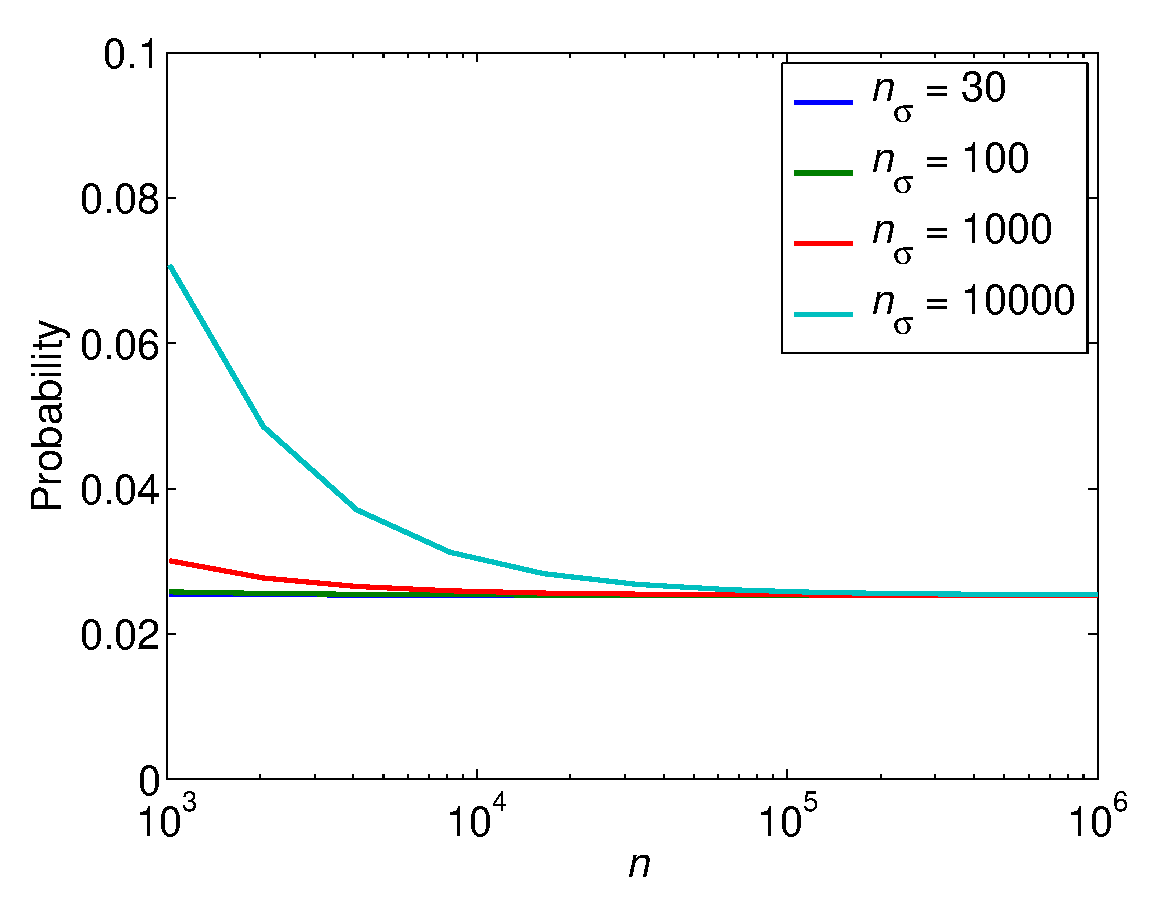
\includegraphics[width=3in]{probfailfig.eps}
\caption{The upper bound on the probability that $\hv_n \ge \hsigma^2$ in \eqref{probfail} for $\alpha_1 = 1 - \sqrt{95\%} \approx 2.5\%$ and $L=1.5$. \label{probfailfig}}
\end{figure}

\end{document}
